\section{Specifica della componente View}\label{view.client} {
%solo client

La componente View si occupa di interagire con l'utente mettendogli a disposizione un'interfaccia (GUI\g) tramite la quale egli può immettere dati, visualizzare informazioni relative al proprio profilo e gestire le chiamate. La View invia al Presenter le richieste di elaborazione dei dati e riceve da quest'ultimo le richieste di aggiornamento dell'interfaccia utente.\\
\`E formata dalle classi:
\begin{itemize}
	\item[] \texttt{mytalk.client.iView.iUser.ICallManage} (sez. \ref{ssub:ICallManage})
	\item[] \texttt{mytalk.client.iView.iUser.ICommunicationView} (sez. \ref{ssub:ICommunicationView})
	\item[] \texttt{mytalk.client.iView.iUser.ILogUser} (sez. \ref{ssub:ILogUser})
	\item[] \texttt{mytalk.client.iView.iUser.IMakeCall} (sez. \ref{ssub:IMakeCall})
	\item[] \texttt{mytalk.client.iView.iUser.IMediaManage} (sez. \ref{ssub:IMediaManage})
	\item[] \texttt{mytalk.client.iView.iUser.IModifyDataUser} (sez. \ref{ssub:IModifyDataUser})
	\item[] \texttt{mytalk.client.iView.iUser.IPageUserView} (sez. \ref{ssub:IPageUserView})
	\item[] \texttt{mytalk.client.iView.iUser.IRegister} (sez. \ref{ssub:IRegister})
	\item[] \texttt{mytalk.client.iView.iUser.IShowDataUser} (sez. \ref{ssub:IShowDataUser})
	\item[] \texttt{mytalk.client.iView.iUser.IUserDataView} (sez. \ref{ssub:IUserDataView})
	\item[] \texttt{mytalk.client.view.user.CallManage} (sez. \ref{ssub:CallManage})
	\item[] \texttt{mytalk.client.view.user.CommunicationView} (sez. \ref{ssub:CommunicationView})
	\item[] \texttt{mytalk.client.view.user.LogUser} (sez. \ref{ssub:LogUser})
	\item[] \texttt{mytalk.client.view.user.MakeCall} (sez. \ref{ssub:MakeCall})
	\item[] \texttt{mytalk.client.view.user.MediaManage} (sez. \ref{ssub:MediaManage})
	\item[] \texttt{mytalk.client.view.user.ModifyDataUser} (sez. \ref{ssub:ModifyDataUser})
	\item[] \texttt{mytalk.client.view.user.PageUserView} (sez. \ref{ssub:PageUserView})
	\item[] \texttt{mytalk.client.view.user.Register} (sez. \ref{ssub:Register})
	\item[] \texttt{mytalk.client.view.user.ShowDataUser} (sez. \ref{ssub:ShowDataUser})
	\item[] \texttt{mytalk.client.view.user.UserDataView} (sez. \ref{ssub:UserDataView})
	\item[] \texttt{mytalk.client.iView.iAdministrator.ILogAdmin} (sez. \ref{ssub:ILogAdmin})
	\item[] \texttt{mytalk.client.iView.iAdministrator.IPageAdminView} (sez. \ref{ssub:IPageAdminView})
	\item[] \texttt{mytalk.client.iView.iAdministrator.IStatisticView} (sez. \ref{ssub:IStatisticView})
	\item[] \texttt{mytalk.client.view.administrator.LogAdmin} (sez. \ref{ssub:LogAdmin})
	\item[] \texttt{mytalk.client.view.administrator.PageAdminView} (sez. \ref{ssub:PageAdminView})
	\item[] \texttt{mytalk.client.view.administrator.StatisticView} (sez. \ref{ssub:StatisticView})
\end{itemize}


\begin{sloppypar}
	\subsection{Package mytalk.client.iView.iUser}{
	
	\begin{figure}[h!tbp]
		\centering
		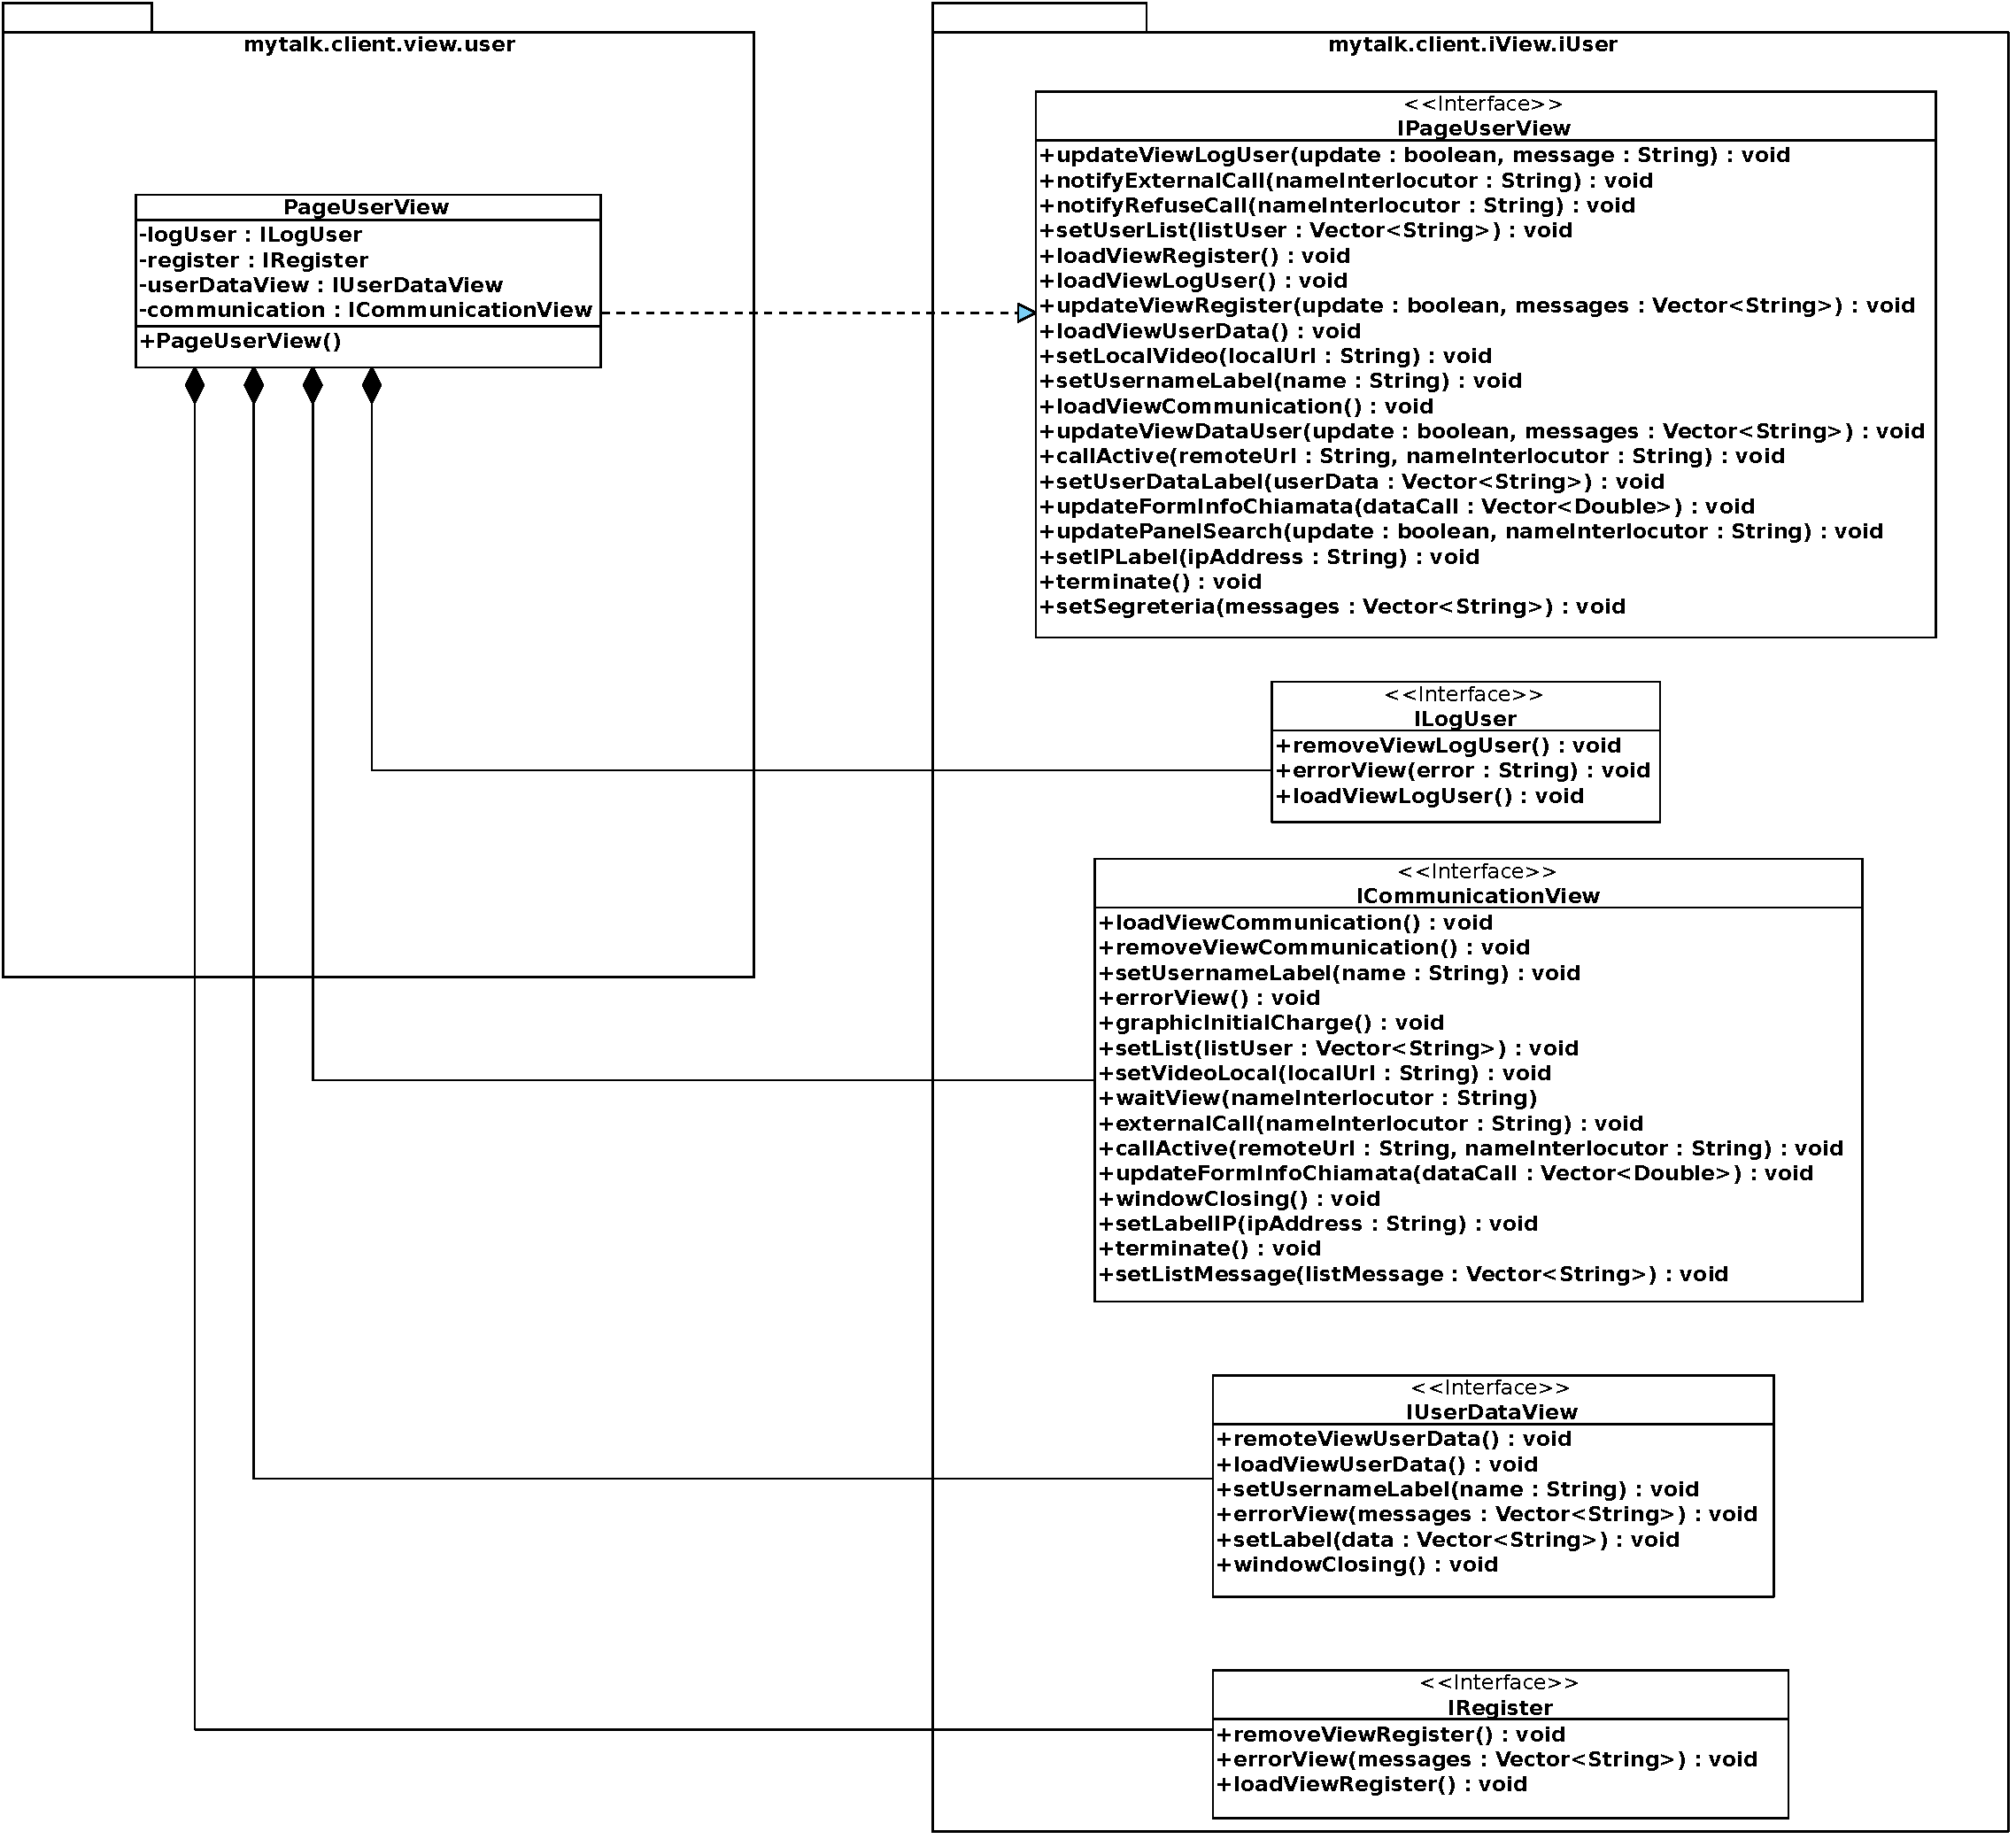
\includegraphics[scale=0.45]{\docsImg classi/pageUserView.pdf}
		\caption{Diagramma delle classi dei package \nolinkurl{mytalk.client.iView.iUser} e \nolinkurl{mytalk.client.view.user}; dettaglio delle classi \nolinkurl{IPageUserView},  \nolinkurl{ILogUser}, \nolinkurl{ICommunicationView}, \nolinkurl{IUserDataView},  \nolinkurl{IRegister} e \nolinkurl{PageUserView}.}
	\end{figure}

	\begin{figure}[h!tbp]
		\centering
		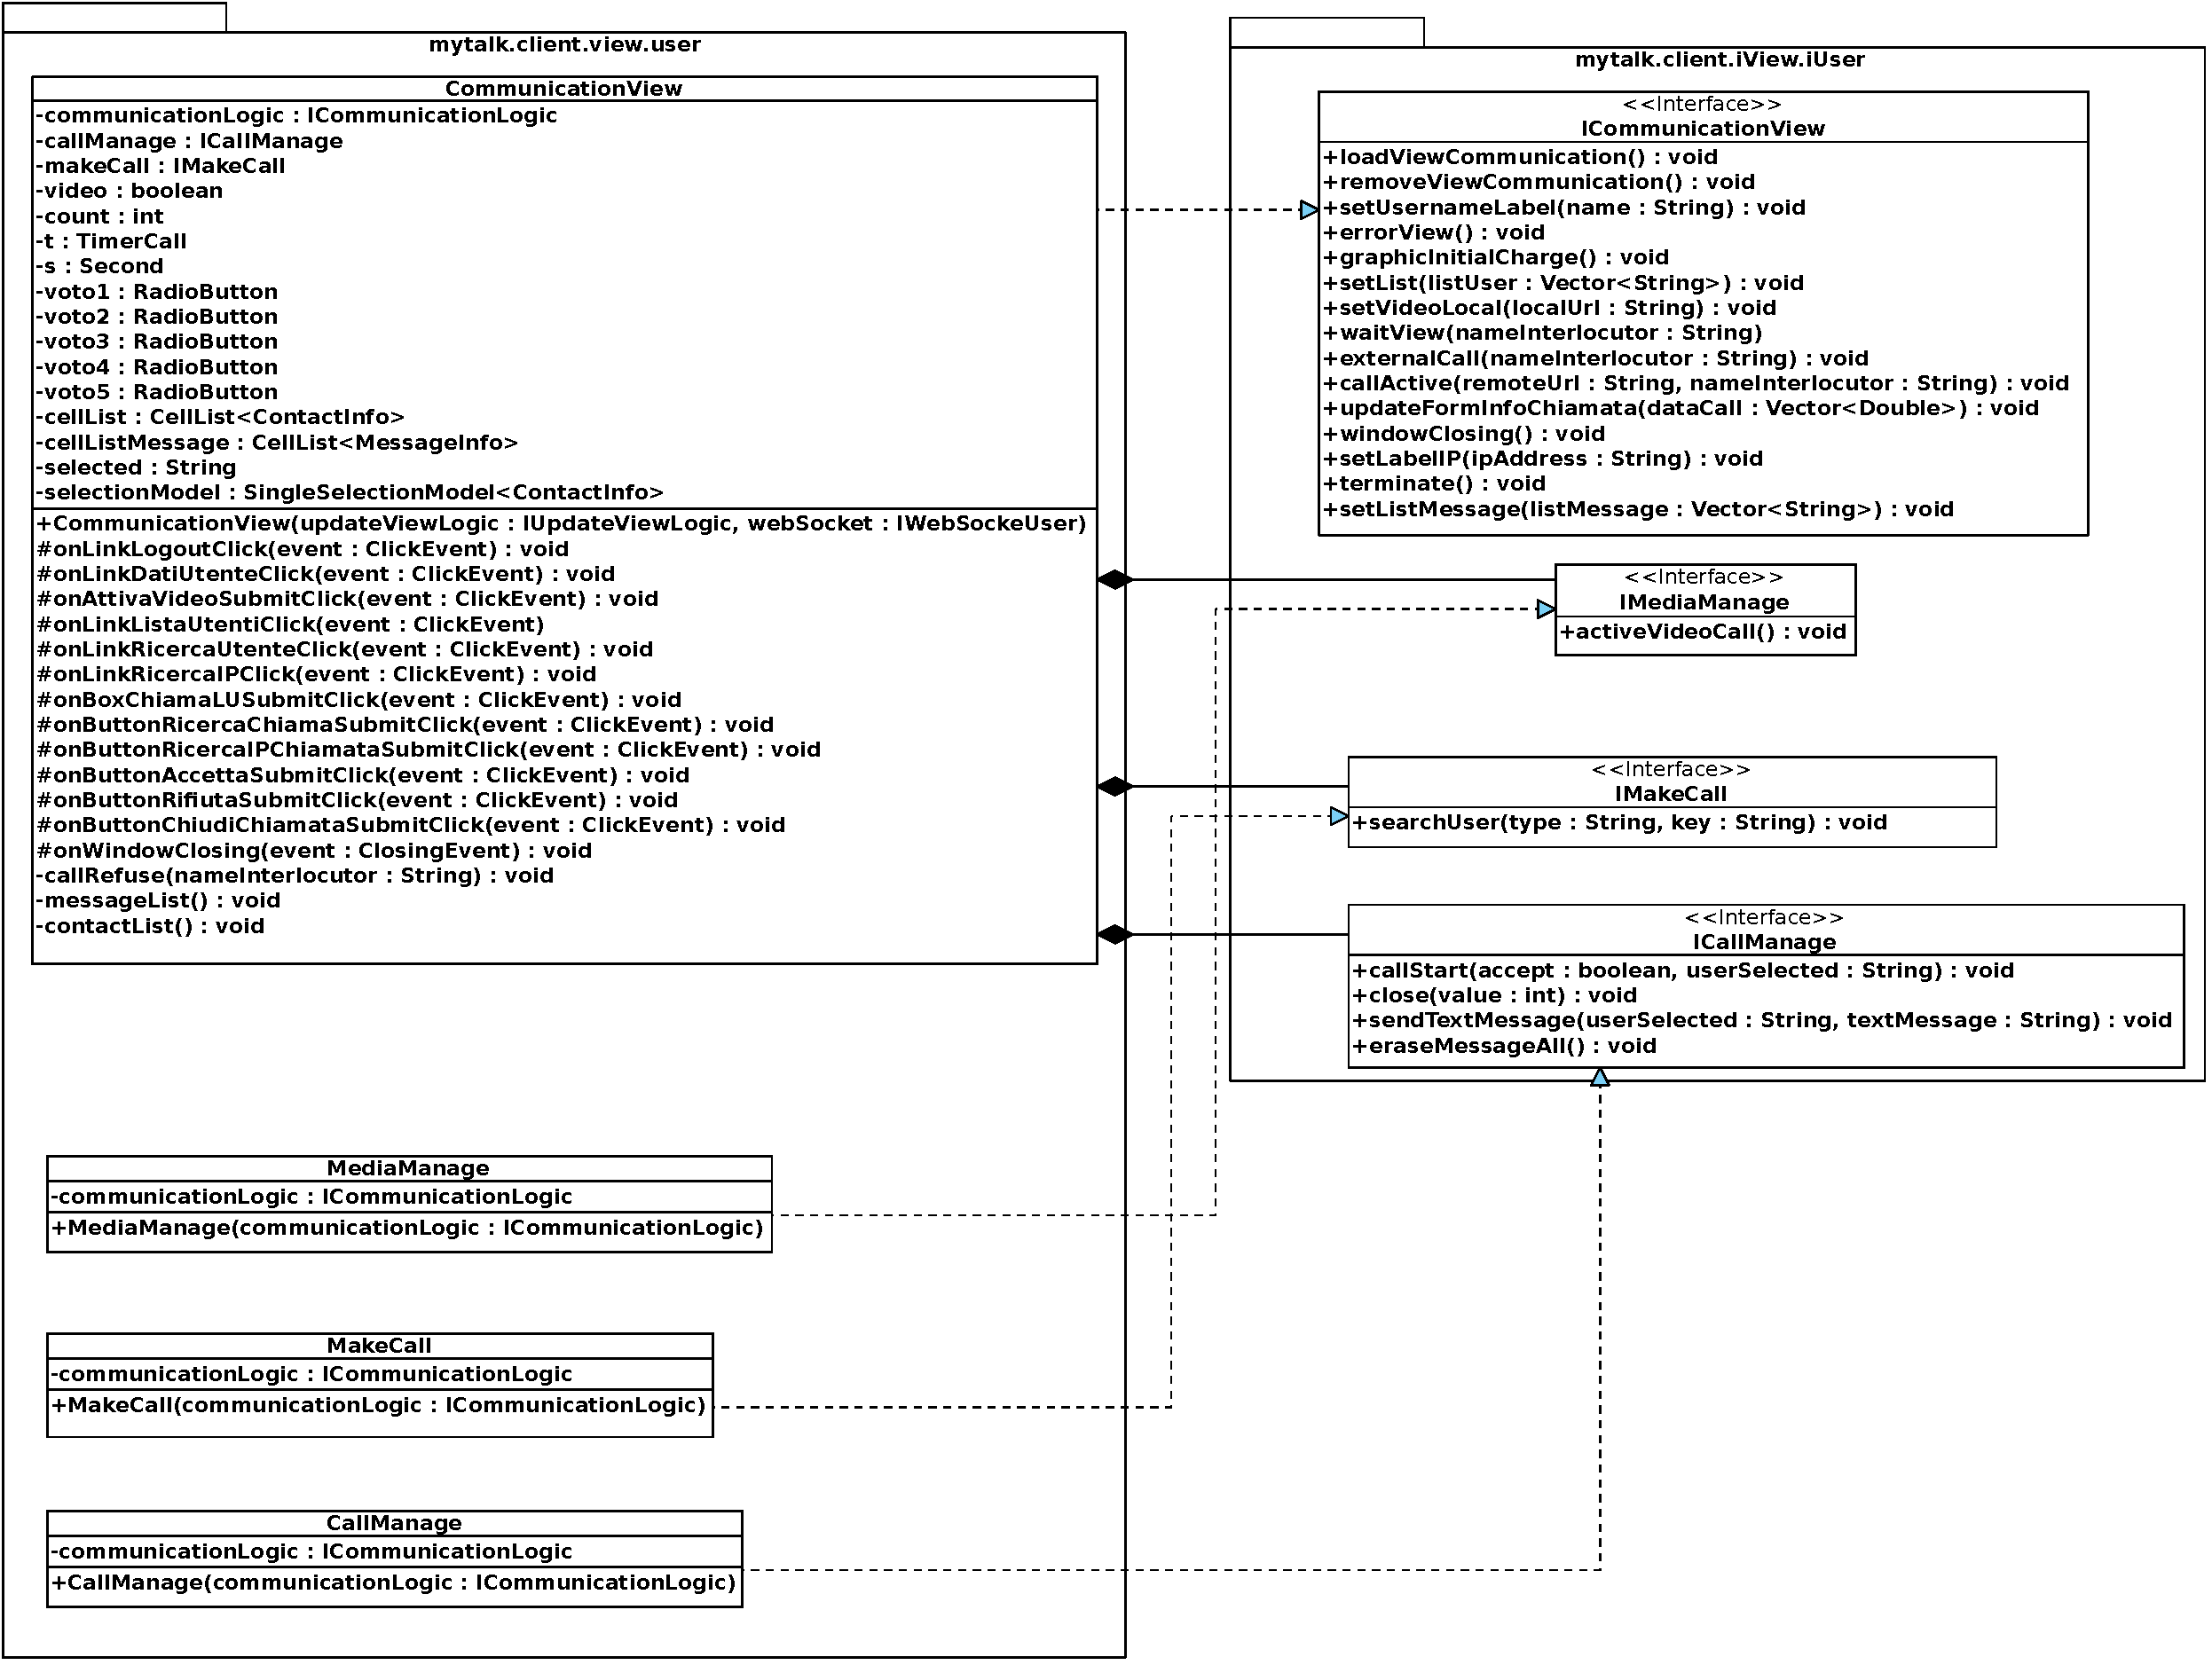
\includegraphics[scale=0.4]{\docsImg classi/viewUserCommunication.pdf}
		\caption{Diagramma delle classi dei package \nolinkurl{mytalk.client.iView.iUser} e \nolinkurl{mytalk.client.view.user}; dettaglio delle classi \nolinkurl{ICommunicationView}, \nolinkurl{IMediaManage}, \nolinkurl{IMakeCall}, \nolinkurl{ICallManage}, \nolinkurl{CommunicationView}, \nolinkurl{MediaManage}, \nolinkurl{MakeCall} e \nolinkurl{CallManage}.}
	\end{figure}
	
	\begin{figure}[h!tbp]
		\centering
		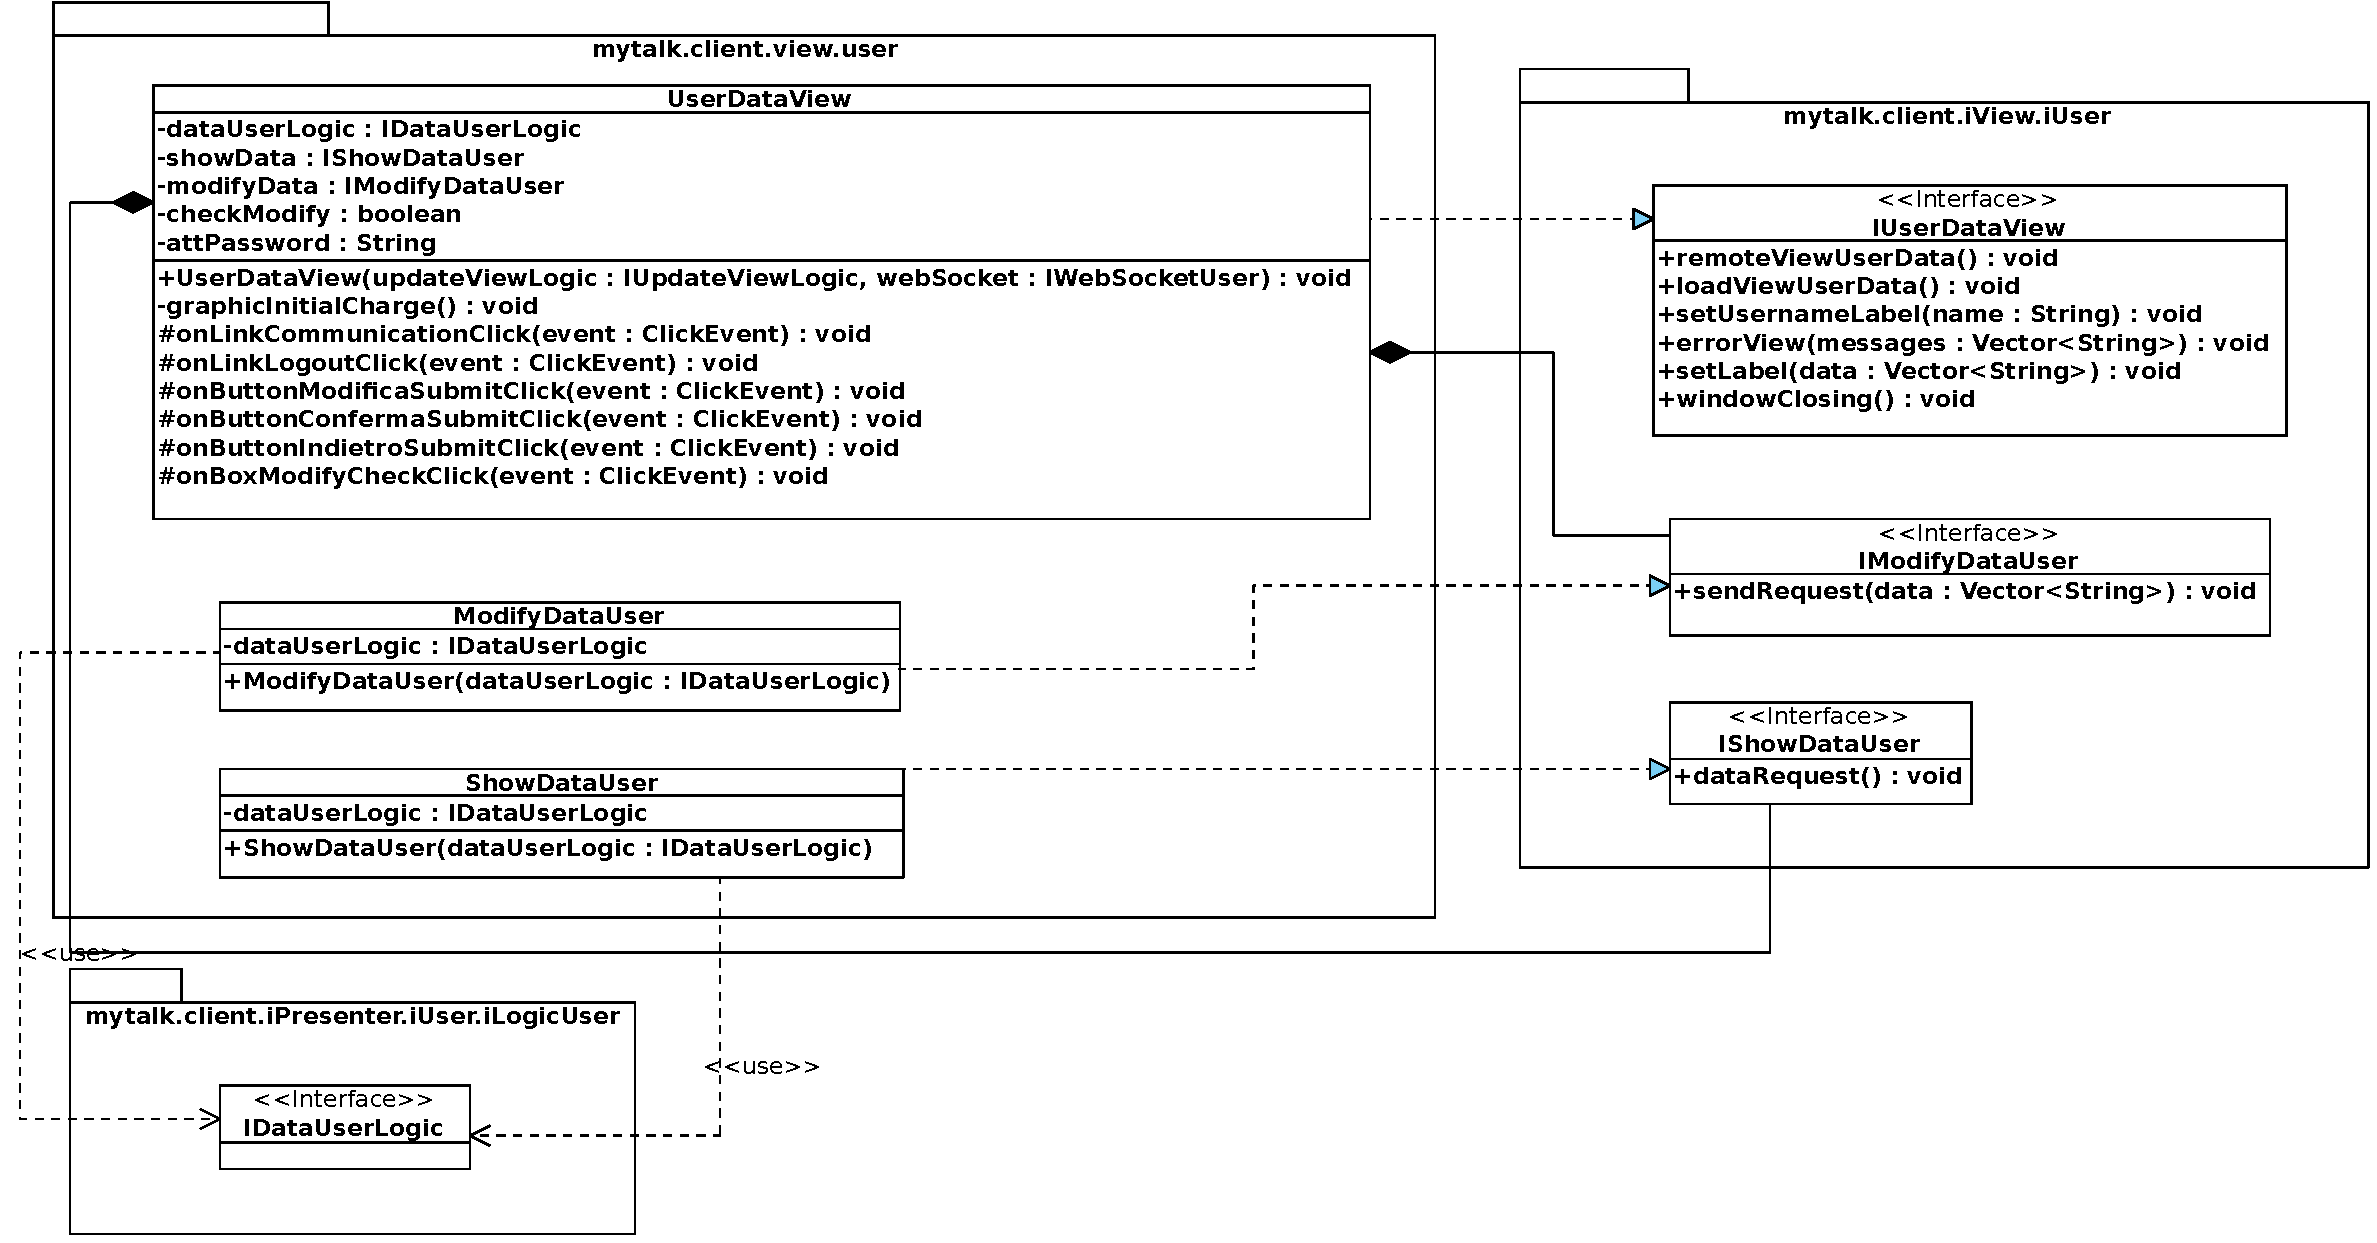
\includegraphics[scale=0.4]{\docsImg classi/UVgestionedatiutente.pdf}
		\caption{Diagramma delle classi dei package \nolinkurl{mytalk.client.iView.iUser} e \nolinkurl{mytalk.client.view.user}; dettaglio delle classi \nolinkurl{IUserDataView}, \nolinkurl{IModifyDataUser}, \nolinkurl{IShowDataUser}, \nolinkurl{UserDataView}, \nolinkurl{ModifyDataUser} e  \nolinkurl{ShowDataUser}.}
	\end{figure}	
	
	\begin{figure}[h!tbp]
		\centering
		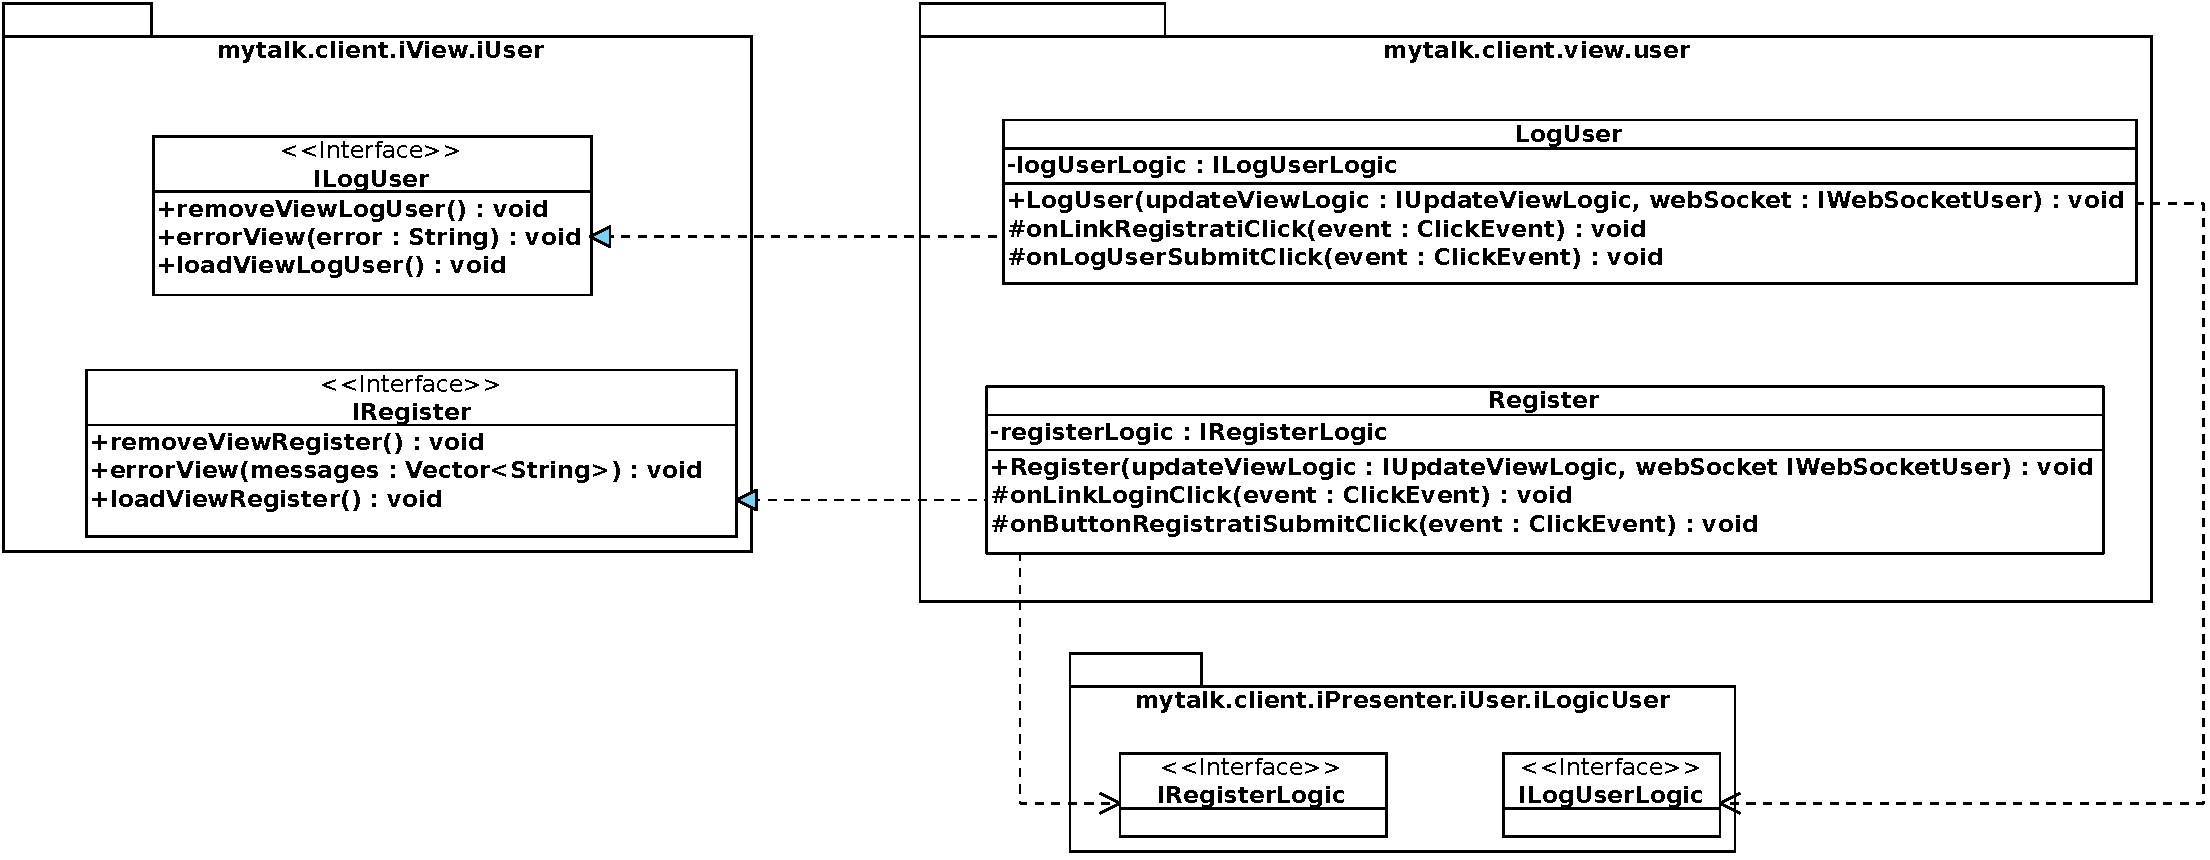
\includegraphics[scale=0.45]{\docsImg classi/regLogin.pdf}
		\caption{Diagramma delle classi dei package \nolinkurl{mytalk.client.iView.iUser} e \nolinkurl{mytalk.client.view.user}; dettaglio delle classi \nolinkurl{ILogUser}, \nolinkurl{IRegister}, \nolinkurl{LogUser} e \nolinkurl{Register}.}
	\end{figure}	
	
	\newpage
				% ICallManage - inizio
		\subsubsection{ICallManage}\label{ssub:ICallManage}{
		\begin{itemize}
			\item[]  \textbf{Funzione:}\\
				Interfaccia che offre operazioni alle classi che compongono la GUI\g~ per la 
				gestione di una comunicazione attiva e interagiscono con essa. L'interfaccia offre inoltre i metodi per l'uso della segreteria.\\
		
			\item[]  \textbf{Relazioni con altre componenti:} \\
				L'interfaccia è implementata da:
				\begin{itemize}
					\item[] \path{mytalk.client.view.user.CallManage}.
				\end{itemize}
				L'interfaccia è utilizzata da:
				\begin{itemize}
					\item[] \path{mytalk.client.view.user.CommunicationView}.\\
				\end{itemize}
					
			\item[]  \textbf{Metodi:}\\
				\texttt{+ void callStart(boolean accept, String userSelected);}\\
				Invia al Presenter, a seconda del valore \texttt{accept}, la richiesta di accettazione o di rifiuto di una 
				comunicazione.\\

				\texttt{+ void close(int value);}\\
				Invia una richiesta al Presenter per chiudere la comunicazione attiva, inviando il 
				valore della valutazione dell'utente.\\
				
				\texttt{+ void sendTextMessage(String userSelected, String textMessage);}\\
				Invia una richiesta al Presenter di invio del messaggio di segreteria verso l'utente selezionato.\\
				
				\texttt{+ void eraseMessageAll();}\\
				Invia una richiesta al presenter per eliminare tutti i messaggi registrati nella segreteria.\\
		\end{itemize}
		}
		% ICallManage - fine
		
		% ICommunicationView - inizio
	\subsubsection{ICommunicationView}\label{ssub:ICommunicationView}{
			\begin{itemize}
				\item[] \textbf{Funzione:} \\ 
					Interfaccia che offre operazioni alle classi che compongono la GUI\g~ della comunicazione e interagiscono con essa.\\

				\item[]  \textbf{Relazioni con altre componenti:} \\
					L'interfaccia è implementata da:
					\begin{itemize}
						\item[] \path{mytalk.client.view.user.CommunicationView}.
					\end{itemize}
					L'interfaccia è utilizzata da
					\begin{itemize}
						\item[] \path{mytalk.client.view.user.PageUserView}.\\
					\end{itemize}

				\item[] \textbf{Metodi:} \\
					\texttt{+ void loadViewCommunication();} \\
					Visualizza la GUI\g~ che permette all'utente di gestire le comunicazioni.\\

					\texttt{+ void removeViewCommunication();} \\
					Nasconde la GUI\g~ di comunicazione.\\

					\texttt{+ void setUsenameLabel(String name);}\\
					Imposta l'etichetta \texttt{LabelUser} con il nome dell'utente autenticato.\\

					\texttt{+ void errorView();}\\
					Imposta e rende visibili i messaggi di errore da segnalare all'utente.\\

					\texttt{+ void graphicInitialCharge();}\\
					Imposta i pannelli da visualizzare e le impostazioni di default. \\

					\texttt{+ void setList(Vector<String> listUser);}\\
					Inserisce gli utenti registrati contenuti nel vettore \texttt{listUser} all'interno del pannello 
					\texttt{ListUser}.\\

					\texttt{+ void setVideoLocal(String localUrl);}\\
					Imposta il video locale con l'indirizzo contenuto nella stringa \texttt{localUrl}.\\

					\texttt{+ void waitView(String nameInterlocutor);}\\
					Visualizza il pannello, per il mittente, in attesa di risposta del destinatario.\\

					\texttt{+ void externalCall(String nameInterlocutor);}\\
					Visualizza il pannello di chiamata in entrata.\\

					\texttt{+ void callActive(String remoteUrl, String nameInterlocutor);}\\
					Visualizza il pannello di informazioni di chiamata ed imposta il video remoto con la stringa 
					\texttt{remoteUrl} e con il nome dell'utente (parametro \texttt{nameInterlocutor}) con cui si è instaurata la comunicazione.\\

					\texttt{+ void updateFormInfoChiamata(Vector<Double> dataCall);}\\
					Visualizza le statistiche delle chiamate contenute nel vettore \texttt{dataCall}.\\

					\texttt{+ void windowClosing();}\\
					Gestisce l'evento di chiusura della finestra della GUI\g~ di comunicazione effettuando il logout e in caso di comunicazione attiva termina la chiamata.\\
					
					\texttt{+ void setLabelIP(String ipAddress);}\\
					Imposta l'etichetta \texttt{LabelIP} con l'indirizzo IP\g~ dell'utente autenticato.\\
					
					\texttt{+ void terminate();}\\
					Metodo che cattura il valore della valutazione dell'utente riguardo la comunicazione in corso. Invia una richiesta di chiusura della comunicazione al Presenter ed, infine, richiama il metodo per tornare alla grafica iniziale.\\
					
					\texttt{+ void setListMessage(Vector<String> listMessage);}\\
					Inserisce i messaggi di segreteria contenuti nel vettore \texttt{listMessage} all'interno del pannello 
					\texttt{ListMessage}.\\
		\end{itemize}			
		}
		% ICommunicationView - fine
		
		
		% ILogUser - inizio
\subsubsection{ILogUser}\label{ssub:ILogUser}{
		\begin{itemize}

			\item[] \textbf{Funzione:}\\
				Offre operazioni alle classi che compongono la GUI\g~ per l'autenticazione degli utenti e interagiscono con essa.\\

			\item[] \textbf{Relazioni con altre componenti:}\\
				L'interfaccia è implementata da:
				\begin{itemize}
					\item[] \path{mytalk.client.view.user.LogUser}.
				\end{itemize}
				L'interfaccia è utilizzata da:
				\begin{itemize}
					\item[] \path{mytalk.client.view.user.PageUserView}.\\
				\end{itemize}

			\item[] \textbf{Metodi:}\\
				\texttt{+ void loadViewLogUser();}\\
				Visualizza la GUI\g~ di autenticazione e seleziona le impostazioni di default\g, i campi vuoti e l'errore (non visibile).\\

				\texttt{+ void removeViewLogUser();}\\
				Nasconde la GUI\g~ di autenticazione.\\

				\texttt{+ void errorView(String error);}\\
				Imposta e rende visibile il messaggio di errore passato dal parametro \texttt{error}.\\
		\end{itemize}
		}
		% ILogUser - fine
		
		
		% IMakeCall - inizio
		\subsubsection{IMakeCall}\label{ssub:IMakeCall}{
		\begin{itemize}
			\item[]  \textbf{Funzione:}
				Interfaccia che offre operazioni alle classi che compongono la 
				GUI\g~ per la gestione della negoziazione di una comunicazione e interagiscono con essa.\\
		
			\item[]  \textbf{Relazioni con altre componenti:} \\
				L'interfaccia è implementata da:
				\begin{itemize}
					\item[] \path{mytalk.client.view.user.MakeCall}.
				\end{itemize}
				L'interfaccia è utilizzata da:
				\begin{itemize}
					\item[] \path{mytalk.client.view.user.CommunicationView}.\\
				\end{itemize}
					
			\item[]  \textbf{Metodi:}\\
				\texttt{+ void searchUser(String type, String key);}\\
				Invia una richiesta al Presenter per cercare e controllare la disponibilità dell'utente 
				desiderato.\\
		\end{itemize}		
		}
		% IMakeCall - fine
		
		\subsubsection{IMediaManage}\label{ssub:IMediaManage}{
		% IMediaManage - inizio
		\begin{itemize}
			\item[]  \textbf{Funzione:}
				Interfaccia che offre operazioni alle classi che compongono la GUI\g~ per la 
				gestione dei media per la comunicazione e interagiscono con essa.\\
		
			\item[]  \textbf{Relazioni con altre componenti:} \\
				L'interfaccia è implementata da:
				\begin{itemize}
					\item[] \path{mytalk.client.view.user.MediaManage}.
				\end{itemize}
				L'interfaccia è utilizzata da:
				\begin{itemize}
					\item[] \path{mytalk.client.view.user.CommunicationView}.\\
				\end{itemize}
					
			\item[]  \textbf{Metodi:}\\
				\texttt{+ void activeVideoLocal();}\\
				Invia una richiesta al Presenter per recuperare l'indirizzo del video locale.\\
		\end{itemize}		
		}
		% IMediaManage - fine
		
		
		% IModifyDataUser - inizio
		\subsubsection{IModifyDataUser}\label{ssub:IModifyDataUser}{
		\begin{itemize}
			\item[] \textbf{Funzione:}\\
				  Offre operazioni alle classi che compongono la GUI\g~ per la modifica dei dati di un utente e interagiscono con essa.\\
				
			\item[] \textbf{Relazioni con altre componenti:}\\
				L'interfaccia è implementata da:
				\begin{itemize}
					\item[] \path{mytalk.client.view.user.ModifyDataUser}. 
				\end{itemize}
				L'interfaccia è utilizzata da:
				\begin{itemize}
					\item[] \path{mytalk.client.view.user.UserDataView}. \\
				\end{itemize}
				
			\item[] \textbf{Metodi:}\\
				\texttt{+ void sendRequest(Vector<String> data);}\\
				Invia una richiesta per sostituire i vecchi dati utente con quelli contenuti nel vettore \texttt{data}.\\
		\end{itemize}		
		}
		% IModifyDataUser - fine
		
		
		% IPageUserView - inizio
		\subsubsection{IPageUserView}\label{ssub:IPageUserView}{
		\begin{itemize}
			\item[] \textbf{Funzione:} \\
			Interfaccia che offre operazioni alle classi che compongono la GUI\g~ e interagiscono con essa.\\
			
			\item[] \textbf{Relazioni con altre componenti:} \\
			L'interfaccia è implementata da:
			\begin{itemize}
				\item[] \path{mytalk.client.view.user.PageUserView}.
			\end{itemize}
			L'interfaccia è utilizzata da:
			\begin{itemize}
				\item[] \path{mytalk.client.presenter.user.logicUser.CommunicationLogic};
				\item[] \path{mytalk.client.presenter.user.logicUser.UpdateUserView}.\\
			\end{itemize}
			
			\item[]  \textbf{Metodi:}\\
			\texttt{+ void updateViewLogUser(boolean update, String message);}\\
			Aggiorna la GUI\g~ a seconda del valore \texttt{update}:
			\begin{itemize}
				\item[-] se \texttt{false}: aggiorna la GUI\g~ di autenticazione visualizzando l'errore opportuno contenuto in \texttt{message};
				\item[-] se \texttt{true}: rende invisibile la GUI\g~ di autenticazione e visualizza la GUI\g~ di comunicazione.\\
			\end{itemize}
			
			\texttt{+ void notifyExternalCall(String nameInterlocutor);}\\
			Notifica alla GUI\g~ di comunicazione l'arrivo di una richiesta di chiamata esterna.\\
			
			\texttt{+ void notifyRefuseCall(String nameInterlocutor);}\\
			Notifica alla GUI\g~ di comunicazione il rifiuto di una richiesta di chiamata.\\
			
			\texttt{+ void setUserList(Vector<String> listUser);}\\
			Imposta la lista dei possibili utenti (parametro \texttt{listUser}) con i quali instaurare una chiamata nella GUI\g~ di comunicazione.\\

			\texttt{+ void loadViewRegister();}\\
			Richiede la visualizzazione della GUI\g~ di registrazione.\\

			\texttt{+ void loadViewLogUser();}\\
			Richiede  la visualizzazione della GUI\g~ di autenticazione.\\

			\texttt{+ void updateViewRegister(boolean update, Vector<String> messages);}\\
			Aggiorna la GUI\g~ a seconda del valore \texttt{update}:
			\begin{itemize}
				\item[-] se \texttt{false}: aggiorna la GUI\g~ di registrazione visualizzando gli errori opportuni contenuti in \texttt{messages}.
				\item[-] se \texttt{true}: rende invisibile la GUI\g~ di registrazione e visualizza la GUI\g~ di autenticazione.\\
			\end{itemize}

			\texttt{+ void loadViewUserData();}\\
			Richiede la visualizzazione della GUI\g~ di gestione dei dati dell'utente.\\

			\texttt{+ void setLocalVideo(String localUrl);}\\
			Invia l'indirizzo del video locale (parametro \texttt{localUrl}) alla GUI\g~ di comunicazione.\\

			\texttt{+ void setUsernameLabel(String name);}\\
			Invia il nome utente (parametro \texttt{name}) alla GUI\g~ di comunicazione e alla GUI\g~ di gestione dei dati dell'utente.\\

			\texttt{+ void loadViewCommunication();}\\
			Richiede la visualizzazione della GUI\g~ di comunicazione.\\

			\texttt{+ void updateViewDataUser(boolean update, Vector<String> messages);}\\
			Aggiorna la GUI\g~ a seconda del valore \texttt{update}:
			\begin{itemize}
				\item[-] se \texttt{false}: aggiorna la GUI\g~ di modifica dei dati dell'utente visualizzando gli errori opportuni contenuti in \texttt{messages};
				\item[-] se \texttt{true}: visualizza il pannello di visualizzazione dei dati dell'utente.\\
			\end{itemize}

			\texttt{+ void setUserDataLabel(Vector<String> userData);}\\
			Invia l'elenco dei dati dell'utente alla GUI\g~ di visualizzazione dei dati.\\

			\texttt{+ void callActive(String remoteUrl, String nameInterlocutor);}\\
			Notifica alla GUI\g~ di comunicazione l'inizio di una conversazione, inviandole l'indirizzo del video remoto (parametro \texttt{remoteUrl}) e lo username (parametro \texttt{nameInterlocutor}) dell'utente remoto.\\

			\texttt{+ void updateFormInfoChiamata(Vector<Double> dataCall);}\\
			Invia i dati delle statistiche alla GUI\g~ di comunicazione.\\

			\texttt{+ void updatePanelSearch(boolean update, String nameInterlocutor);}\\
			Aggiorna la GUI\g~ a seconda del valore \texttt{update}:
			\begin{itemize}
				\item[-] se \texttt{false}: visualizza il pannello di attesa di risposta da parte dell'utente in fase di negoziazione;
				\item[-] se \texttt{true}: aggiorna la GUI\g~ di comunicazione visualizzando l'errore opportuno.\\
			\end{itemize}
			\texttt{+ void setIPLabel(String ipAddress);}\\
			Invia l'indirizzo IP\g~ (parametro \texttt{ipAddress}) alla GUI\g~ di comunicazione.\\
			
			\texttt{+ void terminate();}\\
			Invia alla GUI\g~ di comunicazione un segnale di richiesta di chiusura di conversazione.\\
			
			\texttt{+ void setSegreteria(Vector<String> messagges);}\\
			Imposta la lista dei messaggi in segreteria (parametro \texttt{messagges}) nella GUI\g~ di comunicazione.\\
		\end{itemize}
		}
		% IPageUserView - fine


		% IRegister - inizio
		\subsubsection{IRegister}\label{ssub:IRegister}{
		\begin{itemize}
			\item[] \textbf{Funzione:}\\
				Offre operazioni alle classi che compongono la GUI\g~ per la registrazione di nuovi utenti e interagiscono con essa.\\
				
			\item[] \textbf{Relazioni con altre componenti:}\\
				L'interfaccia è implementata da:
				\begin{itemize}
					\item[] \path{mytalk.client.view.user.Register}. 
				\end{itemize}
				L'interfaccia è utilizzata da:
				\begin{itemize}
					\item[] \path{mytalk.client.view.user.PageUserView}.\\
				\end{itemize}
				
			\item[] \textbf{Metodi:}\\
				\texttt{+ void loadViewRegister();}\\
				Visualizza la GUI\g~ di registrazione.\\
				
				\texttt{+ void removeViewRegister();}\\
				Nasconde la GUI\g~ di registrazione.\\
				
				\texttt{+ void errorView(Vector<String> messages);}\\
				Imposta e rende visibili i messaggi di errore, definiti nel vettore \texttt{messages}, da segnalare all'utente.\\
		\end{itemize}
		}
		% IRegister - fine
		
		
		% IShowDataUser - inizio
		\subsubsection{IShowDataUser}\label{ssub:IShowDataUser}{
		\begin{itemize}
			\item[] \textbf{Funzione:}\\
				  Offre operazioni alle classi che compongono la GUI\g~ per la visualizzazione dei dati di un utente e interagiscono con essa.\\
				
			\item[] \textbf{Relazioni con altre componenti:}\\
				L'interfaccia è implementata da:
				\begin{itemize}
					\item[] \path{mytalk.client.view.user.ShowDataUser}.
				\end{itemize}
				L'interfaccia è utilizzata da:
				\begin{itemize}
					\item[] \path{mytalk.client.view.user.UserDataView}.\\
				\end{itemize}
				
			\item[] \textbf{Metodi:}\\
				\texttt{+ void dataRequest();}\\
				Invia una richiesta al Presenter per recuperare i dati relativi all'utente.\\
		\end{itemize}
		}
		% IShowDataUser - fine
		
		% IUserDataView - inizio
		\subsubsection{IUserDataView}\label{ssub:IUserDataView}{
		\begin{itemize}
			\item[] \textbf{Funzione:}\\
				  Offre operazioni alle classi che compongono la GUI\g~ per la gestione dei dati di un utente e interagiscono con essa.\\
				
			\item[] \textbf{Relazioni con altre componenti:}\\
				L'interfaccia è implementata da:
				\begin{itemize}
					\item[] \path{mytalk.client.view.user.UserDataView}.
				\end{itemize}
				L'interfaccia è utilizzata da:
				\begin{itemize}
					\item[] \path{mytalk.client.view.user.PageUserView}.\\
				\end{itemize}
				
			\item[] \textbf{Metodi:}\\
				\texttt{+ void loadViewUserData();}\\
				Visualizza la GUI\g~ che permette all'utente di visualizzare i propri dati.\\
				
				\texttt{+ void removeViewUserData();}\\
				Nasconde la GUI\g~ di visualizzazione e modifica dati.\\
				
				\texttt{+ void errorView(Vector<String> messages);}\\
				Imposta e rende visibili i messaggi di errore, definiti nel vettore \texttt{messages}, da segnalare all'utente.\\
				
				\texttt{+ void setUsenameLabel(String name);}\\
				Imposta l’etichetta \texttt{LabelUser} con il nome dell’utente autenticato.\\
				
				\texttt{+ void setLabel(Vector<String> data);}\\
				Imposta i campi dei dati dell'utente estrapolati dal vettore \texttt{data}.\\
				
				\texttt{+ void windowClosing();}\\
				Gestisce l'evento di chiusura della finestra della GUI\g~ di gestione dei dati utente effettuando il logout.\\
		\end{itemize}
		}
		% IUserDataView - fine
		
	}
	
	\subsection{Package mytalk.client.view.user} {

		% CallManage - inizio
		\subsubsection{CallManage}\label{ssub:CallManage}{
		\begin{itemize}
			\item[]  \textbf{Funzione:} La classe ha il compito di inoltrare al Presenter le richieste per la gestione di una comunicazione attiva.\\
				
			\item[]  \textbf{Relazioni con altre componenti:} \\
				Implementa l'interfaccia:
				\begin{itemize}
					\item \path{mytalk.client.iView.iUser.ICallManageUser}.
				\end{itemize}
				Usa le classi:
				\begin{itemize}
					\item \path{mytalk.client.presenter.user.logicUser.CommunicationLogic}.
				\end{itemize}
				Tramite le interfacce:
				\begin{itemize}
					\item \path{mytalk.client.iPresenter.iUser.iLogicUser.ICommunicationLogic}.\\
				\end{itemize}
					
			\item[] \textbf{Attributi:}\\
				\texttt{- ICommunicationLogic communicationLogic}: riferimento alla classe \texttt{CommunicationLogic}.\\
				
			\item[] \textbf{Metodi:}\\
				\texttt{+ CallManage(IComunicationLogic communicationLogic);}\\
				Costruttore: inizializza \texttt{communicationLogic} con il valore ricevuto come parametro.\\

				\texttt{+ void callStart(boolean accept, String userSelected);}\\
				Invia al Presenter, a seconda del valore \texttt{accept}, la richiesta di accettazione o di rifiuto di una 
				comunicazione. Se \texttt{accept} è \texttt{true} richiama, attraverso il riferimento \texttt{communicationLogic}, il metodo \texttt{accept(userSelected)}. In caso contrario richiama \texttt{refuse(userSelected)}.\\

				\texttt{+ void close(int value);}\\
				Invia una richiesta al Presenter per chiudere la comunicazione attiva, inviando il valore della 
				valutazione dell'utente.\\
				
				\texttt{+ void sendTextMessage(String userSelected, String textMessage);}\\
				Invia una richiesta al Presenter per inviare il messaggio inserito nel parametro \texttt{textMessage} all'utente indicato nel parametro \texttt{userSelected}.\\
				
				\texttt{+ void eraseMessageAll();}\\
				Invia una richiesta al Presenter per eliminare tutti i messaggi presenti in segreteria.\\
				
		\end{itemize}
		}
		% CallManage - fine

		% CommunicationView - inizio
		\subsubsection{CommunicationView}\label{ssub:CommunicationView}{
			\begin{itemize}
				\item[]  \textbf{Funzione:} \\
				La classe ha il compito di:
				\begin{itemize}
					\item[-] aggiornare opportunamente la GUI\g~ di comunicazione;
					\item[-] gestire gli eventi che l'utente o il sistema possono innescare: inoltra 
					le richieste di comunicazione all'interfaccia \texttt{IMakeCall}, gestisce 
					gli eventi di comunicazione attraverso \texttt{ICallManage} e inoltra gli 
					eventi che gestiscono il video e l'audio a \texttt{IMediaManage};
					\item[-] gestire i link presenti nella pagina.\\
				\end{itemize}

				\item[]  \textbf{Relazioni con altre componenti:} \\
				Implementa l'interfaccia:
				\begin{itemize}
					\item[] \path{mytalk.client.iView.iUser.ICommunicationView}.
				\end{itemize}

				Usa le classi:
				\begin{itemize}
					\item[] \path{mytalk.client.view.user.MediaManage};
					\item[] \path{mytalk.client.view.user.CallManage};
					\item[] \path{mytalk.client.view.user.MakeCall};
					\item[] \path{mytalk.client.presenter.user.logicUser.CommunicationLogic}.
				\end{itemize}
			
				Tramite le interfacce:
				\begin{itemize}
					\item[] \path{mytalk.client.iView.iUser.IMediaManage};
					\item[] \path{mytalk.client.iView.iUser.ICallManage};
					\item[] \path{mytalk.client.iView.iUser.IMakeCall};
					\item[] \path{mytalk.client.iPresenter.iUser.iLogicUser.ICommunicationLogic}.\\
				\end{itemize}

				\item[]  \textbf{Attributi:} \\

					\texttt{- ICommunicationLogic communicationLogic}: riferimento alla classe 
						\texttt{CommunicationLogic}.\\

					\texttt{- ICallManage callManage}: riferimento alla classe \texttt{CallManager}.\\

					\texttt{- IMakeCall makeCall}: riferimento alla classe \texttt{MakeCall}.\\

					\texttt{- IMediaManage mediaManage}: riferimento alla classe \texttt{MediaManager}.\\

					\texttt{- boolean video}: valore booleano che indica lo stato di attivazione del video.	\\

					\texttt{- int count}: valore per contare il numero di richieste di conversazione.\\

					\texttt{- TimerCall t}: timer che effettua un conto alla rovescia per l'attesa della risposta 
						al momento dell'invio di una richiesta di comunicazione.\\
						
					\texttt{- Second s}: timer che simula la funzione di un cronometro durante una comunicazione.\\

					\texttt{- RadioButton voto1}: radio button per assegnare un giudizio di 1.\\

					\texttt{- RadioButton voto2}: radio button per assegnare un giudizio di 2.\\

					\texttt{- RadioButton voto3}: radio button per assegnare un giudizio di 3.\\

					\texttt{- RadioButton voto4}: radio button per assegnare un giudizio di 4.\\

					\texttt{- RadioButton voto5}: radio button per assegnare un giudizio di 5.\\
					
					\texttt{- CellList<ContactInfo> cellList}: oggetto lista di celle contenente le informazioni dei contatti.\\

					\texttt{- CellList<MessageInfo> cellListMessage}: oggetto lista di celle contenente le informazioni dei messaggi.\\
					
					\texttt{- String selected}: stringa contenente lo username dell'utente attualmente selezionato, se nessun utente è selezionato \texttt{selected} risulta vuota.\\
					
					\texttt{- SingleSelectionModel<ContactInfo> selectionModel}: oggetto che indica l'elemento dei \texttt{ContactInfo} attualmente selezionato.\\
					
				\item[] \textbf{Oggetti:}\\
					\texttt{@UiField HTMLPanel MyDiv}: pannello contenente \texttt{DivVideoCommunication} e 
						\texttt{DivPanelControl}.\\

					\texttt{@UiField HTMLPanel DivVideoCommunication}: pannello contenente \texttt{DivVideo},
						   \texttt{DivVideoLocal} e \texttt{FormActivateLocalVideo}.\\

					\texttt{@UiField HTML DivVideo}: codice HTML\g~ per la grafica del video remoto, attivo 
						e inattivo.\\

					\texttt{@UiField HTML DivVideoLocal}: codice HTML\g~ per la grafica del video locale, 
						attivo e inattivo.\\
					
					\texttt{@UiField HTMLPanel FormActivateLocalVideo}: pannello contenente \texttt{AttivaVideoSubmit}.\\

					\texttt{@UiField PushButton AttivaVideoSubmit}: bottone per l'attivazione del video 
						locale.\\

					\texttt{@UiField HTMLPanel DivPanelControl}: pannello contenente \texttt{LinkDatiUtente}, 
					\texttt{LinkLogout}, \texttt{LabelUser}, \texttt{TabBar}, \texttt{FormListaUtenti}, 
					\texttt{FormRicercaUtente}, \texttt{FormRicercaIP}, \texttt{FormMessaggi}, \texttt{FormRicezioneChiamata}, 
					\texttt{FormInfoChiamata} e \texttt{CaptionChiamataInCorso}.\\
					
					\texttt{@UiField InlineHyperlink LinkDatiUtente}: link per passare alla GUI\g~ di 
						gestione dati utente.\\

					\texttt{@UiField InlineHyperlink LinkLogout}: link per passare alla GUI\g~ 
						dell'autenticazione effettuando il logout.\\

					\texttt{@UiField InlineLabel LabelUser}: label che visualizza lo username dell'utente 
						autenticato.\\

					\texttt{@UiField Grid TabBar}: griglia contenente \texttt{LinkListaUtenti}, 
						\texttt{LinkRicercaUtente}, \texttt{LinkRicercaIP} e \texttt{LinkMessaggi}.\\

					\texttt{@UiField InlineHyperlink LinkListaUtenti}: link per visualizzare 
						\texttt{FormListaUtenti}.\\

					\texttt{@UiField HTMLPanel FormListaUtenti}: pannello contenente \texttt{ListUser}, 
						\texttt{BoxChiamaLUSubmit} e \texttt{ButtonSegreteria}.\\

					\texttt{@UiField HTMLPanel ListUser}: pannello contenente l'oggetto \texttt{cellList}.\\

					\texttt{@UiField PushButton BoxChiamaLUSubmit}: bottone per l'invio della richiesta di 
						comunicazione con relativo controllo di stato dell'utente.\\
					
					\texttt{@UiField PushButton ButtonSegreteria}: bottone per l'invio della richiesta di 
						invio di un messaggio di segreteria verso l'utente selezionato.\\

					\texttt{@UiField InlineHyperlink LinkRicercaUtente}: link per visualizzare
						\texttt{FormRicercaUtente}.\\

					\texttt{@UiField FormPanel FormRicercaUtente}: form contenente \texttt{BoxEMail}, 
						\texttt{LabelErroreRicerca} e \texttt{ButtonRicercaChiamaSubmit}.\\

					\texttt{@UiField TextBox BoxEMail}: campo per l'inserimento dell'e-mail dell'utente 
						con il quale si desidera instaurare una comunicazione.\\

					\texttt{@UiField InlineLabel LabelErroreRicerca}: label che contiene l'errore relativo 
						alla ricerca dell'utente.\\

					\texttt{@UiField PushButton ButtonRicercaChiamaSubmit}: bottone per l'invio della 
						richiesta di comunicazione con relativo controllo di esistenza e di stato.\\

					\texttt{@UiField InlineHyperlink LinkRicercaIP}:  link per visualizzare la 
						\texttt{FormRicercaIP}.\\

					\texttt{@UiField FormPanel FormRicercaIP}: form contenente \texttt{LabelIP}, \texttt{BoxRicercaIP}, 
						\texttt{LabelErroreRicercaIP} e \texttt{ButtonRicercaIPChiamaSubmit}.\\

					\texttt{@UiField InlineLabel LabelIP}: label che contiene l'attuale indirizzo IP\g~ dell'utente.\\
						
					\texttt{@UiField TextBox BoxRicercaIP}: campo per l'inserimento dell'indirizzo IP\g~ 
						dell'utente con il quale si desidera instaurare una comunicazione.\\

					\texttt{@UiField InlineLabel LabelErroreRicercaIP}: label che contiene l'errore 
						relativo alla ricerca dell'utente tramite indirizzo IP\g .\\

					\texttt{@UiField PushButton ButtonRicercaIPChiamaSubmit}: bottone per l'invio della 
						richiesta di comunicazione con relativo controllo di esistenza e di stato tramite indirizzo IP\g .\\

					\texttt{@UiField HTMLPanel FormMessaggi}: pannello contenente \texttt{LabelMessaggi}, \texttt{ListMessage} e \texttt{ButtonEliminaTutti}.\\
					
					\texttt{@UiField HTMLPanel ListMessage}: pannello contenente l'oggetto \texttt{cellListMessage}.\\
					
					\texttt{@UiField PushButton ButtonEliminaTutti}: bottone per l'invio della richiesta dell'eliminazione di tutti i messaggi contenuti nella segreteria.\\
					
					\texttt{@UiField FormPanel FormRicezioneChiamata}: form contenente 
						\texttt{LabelNomeUtente}, \texttt{ButtonAccettaSubmit} e \texttt{ButtonRifiutaSubmit}.\\

					\texttt{@UiField InlineLabel LabelNomeUtente}: label che contiene il nome del mittente 
						della richiesta di chiamata.\\

					\texttt{@UiField PushButton ButtonAccettaSubmit}: bottone per accettare la richiesta 
						di chiamata.\\

					\texttt{@UiField PushButton ButtonRifiutaSubmit}: bottone per rifiutare la richiesta 
						di chiamata.\\

					\texttt{@UiField FormPanel FormInfoChiamata}: pannello contenente 
						\texttt{LabelInfoUtente}, \texttt{LabelDurata}, \texttt{LabelLatenza}, \texttt{LabelByte}, 
						\texttt{LabelPack}, \texttt{LabelLostPack}, \texttt{PanelVote} e \texttt{ButtonChiudiChiamataSubmit}.\\

					\texttt{@UiField InlineLabel LabelInfoUtente}: label che contiene il nome dell'utente 
						coinvolto nella comunicazione.\\

					\texttt{@UiField InlineLabel LabelDurata}: label che contiene la durata della 
						comunicazione.\\

					\texttt{@UiField InlineLabel LabelLatenza}: label che contiene la latenza della 
						comunicazione.\\

					\texttt{@UiField InlineLabel LabelByte}: label che contiene il numero di byte inviati 
						durante la comunicazione.\\

					\texttt{@UiField InlineLabel LabelPack}:  label che contiene il numero di pacchetti 
						inviati durante la comunicazione.\\

					\texttt{@UiField InlineLabel LabelLostPack}: label che contiene il numero di pacchetti 
						persi durante la comunicazione.\\

					\texttt{@UiField HorizontalPanel PanelVote}: pannello orizzontale contenente i 
						\texttt{RadioButton} per ricavare l'informazione del giudizio dell'utente riguardo alla 
						comunicazione effettuata.\\

					\texttt{@UiField PushButton ButtonChiudiChiamataSubmit}: bottone per l'invio della 
						richiesta di chiusura della comunicazione.\\

					\texttt{@UiField CaptionPanel CaptionChiamataInCorso}: pannello contenente \texttt{LabelTimer}.\\

					\texttt{@UiField InlineLabel LabelTimer}: label che indica lo stato di attesa del 
						mittente di una richiesta di chiamata attraverso un conto alla rovescia.\\

			\item[] \textbf{Metodi:}\\
				\texttt{+ CommunicationView(IUpdateViewLogic updateViewLogic, IWebSocketUser webSocket);}\\
				Costruttore: inizializza \texttt{communicationLogic} con i valori ricevuti come 
				parametri, imposta inoltre \texttt{webSocket}, \texttt{makeCall}, \texttt{callManage} e 
				\texttt{mediaManage} con il valore del riferimento \texttt{communicationLogic}. Imposta gli 
				attributi degli oggetti che compongono la GUI\g~ e imposta video a false e count a 0. Imposta 
				invisibili tutte le \texttt{LabelError} e i disabilita i bottoni \texttt{Chiama} e \texttt{Lascia Messaggio}. Inoltre crea gli oggetti \texttt{ListUser} e \texttt{ListMessage}.\\

				\texttt{+ void loadViewCommunication();}\\
				Visualizza la GUI\g~ di comunicazione e richiama i metodi \texttt{graphicInitialCharge()} e attraverso il riferimento \texttt{communicationLogic} richiama \texttt{setUserList()} che crea una richiesta per ottenere la lista degli utenti.\\

				\texttt{+ void removeViewCommunication();}\\
				Nasconde la GUI\g~ di comunicazione.\\

				\texttt{+ void setUsernameLabel(String name);}\\
				Imposta l'etichetta \texttt{LabelUser} con il nome dell'utente autenticato passato attraverso la stringa \texttt{name}.\\

				\texttt{+ void errorView();}\\
				Rende visibili le \texttt{LabelError}\\

				\texttt{+ void graphicInitialCharge()};\\
				Nel caso in cui più richieste di comunicazione siano presenti tale metodo non aggiorna la GUI\g, in caso 
				contrario imposta la GUI\g~ di comunicazione allo stato iniziale. Tale stato è il seguente:
				\begin{itemize}
					\item[-] \texttt{count}: 0
					\item[-] \texttt{timer}: reset
					\item[-] \texttt{TabBar}: visibile
					\item[-] \texttt{LinkListaUtenti}: selezionato
					\item[-] \texttt{FormListaUtenti}: visibile
					\item[-] \texttt{tutte le LabelError}: valori iniziali e invisibili
					\item[-] \texttt{FormRicercaUtente}: invisibile
					\item[-] \texttt{FormRicercaIP}: invisibile
					\item[-] \texttt{CaptionChiamataInCorso}: invisibile
					\item[-] \texttt{FormRicezioneChiamata}: invisibile
					\item[-] \texttt{FormInfoChiamata}: invisibile
					\item[-] \texttt{DivVideo}: HTML immagine di attesa\\
				\end{itemize}

				\texttt{+ void setVideoLocal(String localUrl);}\\
				Imposta il tag \texttt{DivVideoLocal} con il codice HTML\g~ per il video con l'indirizzo passato attraverso la stringa \texttt{localUrl}.
				Inoltre rende invisibile \texttt{FormActivateLocalVideo}, attiva i bottoni \texttt{Chiama} (nel caso della lista utenti solo di quelli online) e imposta video a \texttt{true}.\\

				\texttt{+ void waitView(String nameInterlocutor);}\\
				Rende invisibile \texttt{TabBar}, \texttt{FormListaUtenti}, \texttt{FormRicercaUtente}, \texttt{FormRicercaIP} e \texttt{FormMessaggi}. 
				Rende visibile \texttt{CaptionChiamataInCorso} e fa partire il conto alla rovescia per l'attesa della risposta. 
				Imposta inoltre il nome del destinatario con la stringa \texttt{utente} e incrementa \texttt{count}.\\

				\texttt{- void callRefuse(String nameInterlocutor);}\\
				Se il numero di chiamate in attesa è diverso da 1 allora viene solo decrementato \texttt{count}, altrimenti viene richiamato il metodo \texttt{graphicInitialCharge()} e richiamato attraverso il riferimento \texttt{callManage} il metodo \texttt{callStart(false, nameInterlocutor)} che dichiara che la negoziazione verso l'utente contenuto nel parametro \texttt{nameInterlocutor} è fallita.\\

				\texttt{+ void externalCall(String nameInterlocutor);}\\
				Viene incrementato \texttt{count} (il numero di chiamate in attesa). Se il video è attivo e \texttt{count} vale 1 allora \texttt{TabBar}, \texttt{FormListaUtenti}, \texttt{FormRicercaUtente} e \texttt{FormRicercaIP} vengono resi 
				invisibili, e viene visualizzato \texttt{FormRicezioneChiamata} impostando ad \texttt{nameInterlocutor} il contenuto di \texttt{LabelNomeUtente}. 
				Nel caso in cui il video non sia attivo o il numero di chiamate in attesa sia diverso da 1 allora viene 
				visualizzato un messaggio di errore.\\

				\texttt{+ void callActive(String remoteUrl, String nameInterlocutor);}\\
				Blocca e reimposta il timer. Inoltre rende invisibili \texttt{FormRicezioneChiamata} e \texttt{CaptionChiamataInCorso}. 
				Rende visibile \texttt{FormInfoChiamata} impostando \texttt{LabelInfoUtente} con il parametro \texttt{nameInterlocutor}. Inoltre, 
				imposta il \texttt{DivVideo} con l'indirizzo del video remoto dell'utente remoto contenuto nel parametro \texttt{remoteUrl}.\\

				\texttt{+ void updateFormInfoChiamata(Vector<Double> dataCall);}\\
				Imposta le Label di \texttt{FormInfoChiamata} con i parametri passati nel vettore \texttt{dataCall}.\\

				\texttt{+ void windowClosing();}\\
				Gestisce l'evento di chiusura della finestra della GUI\g~ della comunicazione. Richiama il metodo \texttt{close()} attraverso il riferimento \texttt{callManage} nel caso in cui ci sia una chiamata attiva e
				richiama il metodo \texttt{logoutUser()} attraverso il riferimento \texttt{dataUserLogic}.\\
				
				\texttt{- void contactList();}\\
				Metodo che crea l'oggetto \texttt{cellList} e gli abbina il metodo per la selezione di un singolo elemento all'interno della lista.\\
				
				\texttt{- void messageList();}\\
				Metodo che crea l'oggetto \texttt{cellListMessage} e gli abbina il metodo per la selezione di un singolo elemento all'interno della lista.\\
				
				\texttt{+ void setList(Vector<String> listUser);}\\
				Metodo che popola con il vettore \texttt{listUser} l'oggetto \texttt{cellList}.\\
				
				\texttt{+ void setListMessage(Vector<String> listMessage);}\\
				Metodo che popola con il vettore \texttt{listMessage} l'oggetto \texttt{cellListMessage}  e aggiorna la grafica evidenziando il caso in cui siano arrivati nuovi messaggi.\\
			
				\texttt{+ void setLabelIP(String ipAddress);}\\
				Imposta l'etichetta \texttt{LabelIP} con l'indirizzo IP\g~ dell'utente autenticato passato attraverso la stringa \texttt{ipAddress}.\\
				
				\texttt{+ void terminate();}\\
				Metodo che imposta \texttt{count} a 0 e viene richiamato, attraverso il riferimento \texttt{callManage}, il metodo \texttt{close(value)} che richiede la 
				terminazione della comunicazione inviando il voto dell'utente. Richiama, inoltre, il metodo 
				\texttt{graphicInitialCharge()}.\\
	
			\item[] \textbf{Eventi:}\\
				\texttt{@UiHandler void onLinkDatiUtenteClick(ClickEvent event);}\\
				All'evento \texttt{Click} dell'oggetto \texttt{LinkDataUser} viene richiamato il metodo \texttt{removeViewCommunication()} e attraverso il riferimento \texttt{communicationLogic} richiama \texttt{loadViewDataUser()}. 
				Se sono presenti chiamate attive richiama, attraverso il riferimento \texttt{callManage}, il metodo \texttt{close()} e pone \texttt{count} a 0.\\

				\texttt{@UiHandler void onLinkLogoutClick(ClickEvent event);}\\
				All'evento \texttt{Click} dell'oggetto \texttt{LinkLogout} viene richiamato il metodo
				\texttt{removeViewCommunication()}. Inoltre utilizza il riferimento \texttt{communicationLogic} per 
				effettuare il logout e richiamare la GUI di autenticazione attraverso il metodo \texttt{logoutUser()}. 
				Se sono presenti chiamate attive richiama, attraverso il riferimento \texttt{callManage}, il metodo 
				\texttt{close()} e pone count a 0.\\

				\texttt{@UiHandler void onAttivaVideoSubmitClick(ClickEvent event);}\\
				All'evento \texttt{Click} dell'oggetto \texttt{AttivaVideoSubmit} viene richiamato, attraverso il riferimento 
				\texttt{mediaManage}, il metodo \texttt{activeVideoLocal()}.\\

				\texttt{@UiHandler void onLinkListaUtentiClick(ClickEvent event);}\\
				All'evento \texttt{Click} dell'oggetto \texttt{LinkListaUtenti} viene resa visibile \texttt{FormListaUtenti} e 
				vengono rese invisibili \texttt{FormRicercaUtente}, \texttt{FormRicercaIP} e \texttt{FormMessaggi}.\\

				\texttt{@UiHandler void onLinkRicercaUtenteClick(ClickEvent event);}\\
				All'evento \texttt{Click} dell'oggetto \texttt{LinkRicercaUtente} viene resa visibile la \texttt{FormRicercaUtente} 
				e vengono rese invisibili \texttt{FormListaUtenti}, \texttt{FormRicercaIP} e \texttt{FormMessaggi}.\\

				\texttt{@UiHandler void onLinkRicercaIPClick(ClickEvent event);}\\
				All'evento \texttt{Click} dell'oggetto \texttt{LinkRicercaIP} viene resa visibile la \texttt{FormRicercaIP} e 
				vengono rese invisibili \texttt{FormRicercaUtente}, \texttt{FormListaUtenti} e \texttt{FormMessaggi}.\\

				\texttt{@UiHandler void onLinkMessaggiClick(ClickEvent event);}\\
				All'evento \texttt{Click} dell'oggetto \texttt{LinkMessaggi} viene resa visibile la \texttt{FormMessaggi} e 
				vengono rese invisibili \texttt{FormRicercaUtente}, \texttt{FormListaUtenti} e \texttt{FormRicercaIP}.\\
				
				\texttt{@UiHandler void onBoxChiamaLUSubmitClick(ClickEvent event);}\\
				All'evento \texttt{Click} dell'oggetto \texttt{BoxChiamaLUSubmit}, solo se è stato selezionato un utente online, viene inviata una richiesta di comunicazione all'utente selezionato attraverso il 
				riferimento \texttt{makeCall}, il quale richiama il metodo \texttt{searchUser(String type, String nameInterlocutor)}.\\
				
				\texttt{@UiHandler void onButtonSegreteriaClick(ClickEvent event);}\\
				All'evento \texttt{Click} dell'oggetto \texttt{ButtonSegreteria}, solo se è stato selezionato un utente, rende visibile la finestra di dialogo che permette di creare un messaggio da inviare all'utente selezionato.\\

				\texttt{@UiHandler void onButtonRicercaChiamaSubmitClick(ClickEvent event);}\\
				All'evento \texttt{Click} dell'oggetto \texttt{BoxRicercaChiamaSubmit} viene inviata una 
				richiesta di comunicazione all'utente selezionato attraverso il riferimento \texttt{makeCall} che richiama 
				il metodo \texttt{searchUser(String tipo, String utente)}.\\

				\texttt{@UiHandler void onButtonRicercaIPChiamaSubmitClick(ClickEvent event);}\\
				All'evento \texttt{Click} dell'oggetto \texttt{BoxRicercaIPChiamaSubmit} viene inviata 
				una richiesta di comunicazione all'utente selezionato attraverso il riferimento \texttt{makeCall}, il quale 
				richiama il metodo \texttt{searchUser(String tipo, String utente)}.\\
				
				\texttt{@UiHandler void onButtonEliminaTuttiClick(ClickEvent event);}\\
				All'evento \texttt{Click} dell'oggetto \texttt{ButtonEliminaTutti}, gli elementi presenti all'interno della \texttt{listMessage} e attraverso il riferimento a \texttt{callManage} richiama il metodo \texttt{eraseMessageAll()}.\\

				\texttt{@UiHandler void onButtonAccettaSubmitClick(ClickEvent event);}\\
				All'evento \texttt{Click} dell'oggetto \texttt{ButtonAccettaSubmit} vengono resi invisibili \texttt{FormRicezioneChiamata} 
				e \texttt{CaptionChiamataInCorso}. Inoltre, viene chiamato, attraverso il metodo \texttt{callManage}, il 
				metodo \texttt{callStart(true, utente)} che permette di instaurare la comunicazione.\\

				\texttt{@UiHandler void onButtonRifiutaSubmitClick(ClickEvent event);}\\
				All'evento \texttt{Click} dell'oggetto \texttt{ButtonRifiutaSubmit} chiama il metodo \texttt{graphicInitialCharge()}. 
				Inoltre, viene chiamato, attraverso il metodo \texttt{callManage}, il metodo \texttt{callStart(false, utente)} 
				che permette di rifiutare la comunicazione.\\

				\texttt{@UiHandler void onButtonChiudiChiamataSubmitClick(ClickEvent event);}\\
				All'evento \texttt{Click} dell'oggetto \texttt{ButtonChiudiChiamataSubmit}, \texttt{count} viene impostato a 0 e viene richiamato, attraverso il riferimento \texttt{callManage}, il metodo \texttt{close(value)} che richiede la 
				terminazione della comunicazione inviando il voto dell'utente. Richiama, inoltre, il metodo 
				\texttt{graphicInitialCharge()}.\\

				\texttt{@UiHandler void onWindowClosing(Window.ClosingEvent event);}\\
				Alla chiusura della finestra vengono richiamati, attraverso i riferimenti \texttt{callManage} e 
				\texttt{communicationLogic}, ripettivamente i metodi \texttt{close(0)} e \texttt{logoutUser()}. 
				Il metodo \texttt{close(0)} viene richiamato solo nel caso in cui \texttt{count} sia maggiore di 0.\\
				
			\end{itemize}
		}
		% CommunicationView - fine
		
		% LogUser - inizio
		\subsubsection{LogUser}\label{ssub:LogUser}{
		\begin{itemize}
			\item[] \textbf{Funzione:}\\
				  La classe ha il compito di:
				\begin{itemize}
					\item[-] aggiornare opportunamente la GUI\g~ di autenticazione;
					\item[-] gestire gli eventi che l'utente o il sistema possono innescare inoltrando le richieste all'interfaccia \path{mytalk.client.presenter.user.logicUser.ILogUserLogic};
					\item[-] gestire i link presenti nella pagina.\\
				\end{itemize}
				
			\item[] \textbf{Relazioni con altre componenti:}\\
				Implementa l'interfaccia:
				\begin{itemize}
					\item[] \path{mytalk.client.iView.iUser.ILogUser}. 
				\end{itemize}
				Usa le classi:
				\begin{itemize}
					\item[] \path{mytalk.client.presenter.user.logicUser.LogUserLogic}.
				\end{itemize}
				Tramite le interfacce:
				\begin{itemize}
					\item[] \path{mytalk.client.iPresenter.iUser.iLogicUser.ILogUserLogic}.\\
				\end{itemize}

			\item[] \textbf{Attributi:}\\
				\texttt{- ILogUserLogic logUserLogic;}\\
				Riferimento alla classe \texttt{LogUserLogic}.\\

			\item[] \textbf{Oggetti:}\\
				\texttt{@UiField HTMLPanel MyDivLogin;}\\
				Pannello contente \texttt{FormLogUser} e \texttt{LinkRegistrati}.\\
				
				\texttt{@UiField FormPanel FormLogUser;}\\
				Form contenente \texttt{BoxUtente}, \texttt{BoxPassword}, \texttt{LabelError} e \texttt{LogUserSubmit}.\\
				
				\texttt{@UiField TextBox BoxUtente;}\\
				Campo per l'inserimento del nome utente.\\
				
				\texttt{@UiField TextBox BoxPassword;}\\
				Campo per l'inserimento della password.\\
				
				\texttt{@UiField InlineLabel LabelError;}\\
				Label che in presenza di errore segnala il tipo di errore.\\
				
				\texttt{@UiField PushButton LogUserSubmit;}\\
				Bottone per l'invio della richiesta controllo delle credenziali di autenticazione.\\
				
				\texttt{@UiField InlineHyperlink LinkRegistrati;}\\
				Link per passare alla grafica della registrazione.\\
				
			\item[] \textbf{Metodi:}\\
				\texttt{+ LogUser(IUpdateViewLogic updateViewLogic, IWebSocketUser webSocket);}\\
				Costruttore: inizializza \texttt{logUserLogic} con i valori ricevuti, imposta gli attributi degli oggetti che compongono la GUI\g. Imposta come invisibile \texttt{LabelError}.\\
				
				\texttt{+ void loadViewLogUser();}\\
				Visualizza la GUI\g~ di autenticazione e seleziona le impostazioni di default\g~: \texttt{BoxUtente} e \texttt{BoxPassword} vuoti e \texttt{LabelError} invisibile.\\
				
				\texttt{+ void removeViewLogUser();}\\
				Nasconde la GUI\g~ di login.\\
				
				\texttt{+ void errorView(String error);}\\
				Imposta e rende visibile \texttt{LabelError} inserendo il contenuto della stringa \texttt{error}.\\
				
			\item[] \textbf{Eventi:}\\
				\texttt{@UiHandler void onLinkRegistratiClick(ClickEvent event);}\\
				All'evento \texttt{Click} dell'utente richiama il metodo \texttt{removeViewLogUser()} e, attraverso il riferimento \texttt{logUserLogic}, richiama il metodo \texttt{loadViewRegister()}.\\
				
				\texttt{@UiHandler void onLogUserSubmitClick(ClickEvent event);}\\
				All'evento \texttt{Click} dell'oggetto \texttt{LogUserSubmit} i dati inseriti all'interno dei campi \texttt{BoxUtente} e \texttt{BoxPassword} vengono inseriti in un vettore e inviati attraverso il riferimento \texttt{logUserLogic} al metodo \texttt{validateData(Vector<String>)} per effettuare il controllo dei dati di autenticazione.\\
		\end{itemize}
		}
		% LogUser - fine
		
		% MakeCall - inizio
		\subsubsection{MakeCall}\label{ssub:MakeCall}{
			\begin{itemize}
				\item[]  \textbf{Funzione:} \\
					La classe ha il compito di inoltrare al Presenter le richieste per la gestione della negoziazione 
					di una comunicazione.\\
					
					\item[]  \textbf{Relazioni con altre componenti:} \\
						Implementa l'interfaccia:
						\begin{itemize}
							\item[] \path{mytalk.client.iView.iUser.IMakeCall}.
						\end{itemize}
						Usa le classi:
						\begin{itemize}
							\item[] \path{mytalk.client.presenter.user.logicUser.CommunicationLogic}.
						\end{itemize}
						Tramite le interfacce:
						\begin{itemize}
							\item[] \path{mytalk.client.iPresenter.iUser.iLogicUser.ICommunicationLogic}.
						\end{itemize}
							
					\item[]  \textbf{Attributi:}\\
						\texttt{- ICommunicationLogic communicationLogic}: riferimento alla classe \texttt{CommunicationLogic}.\\
						
					\item[] \textbf{Metodi:}\\
						\texttt{+ MakeCall(IComunicationLogic communicationLogic);}\\
						Costruttore: inizializza \texttt{communicationLogic} con il valore ricevuto come parametro.\\

						\texttt{+ void searchUser(String type, String key);}\\
						Invia una richiesta al Presenter per cercare l'utente desiderato e controllarne la disponibilità. 
						L'attributo \texttt{type} indica in che chiave viene ricercato l'utente e \texttt{key} è la stringa per il confronto con il database\g.\\
			\end{itemize}
			}
		% MakeCall - fine

		% MediaManage - inizio
		\subsubsection{MediaManage}\label{ssub:MediaManage}{
			\begin{itemize}
				\item[]  \textbf{Funzione:} \\
				La classe ha il compito di inoltrare al Presenter le richieste per la gestione dei media per la 
				comunicazione.
				
				\item[]  \textbf{Relazioni con altre componenti:} \\
				Implementa l'interfaccia:
				\begin{itemize}
					\item[] \path{mytalk.client.iView.iUser.IMediaManage}.
				\end{itemize}
				Usa le classi:
				\begin{itemize}
					\item[] \path{mytalk.client.presenter.user.logicUser.CommunicationLogic}.
				\end{itemize}					
				Tramite le interfacce:
				\begin{itemize}
					\item[] \path{mytalk.client.iPresenter.iUser.iLogicUser.ICommunicationLogic}.
				\end{itemize}
				
				\item[]  \textbf{Attributi:}\\
				\texttt{- ICommunicationLogic communicationLogic}: riferimento alla classe \texttt{CommunicationLogic}.\\
				
				\item[]  \textbf{Metodi:}\\
				\texttt{+ MediaManage(IComunicationLogic comunicationLogic);}\\
				Costruttore: inizializza \texttt{CommunicationLogic} con il valore ricevuto come parametro.\\

				\texttt{+ void activeVideoLocal();}\\
				Invia una richiesta al Presenter attraverso il metodo \texttt{getLocalUrl()} per recuperare l'indirizzo del 
				video locale.\\
			\end{itemize}
			}
		% MediaManage - fine

		% ModifyDataUser - inizio
		\subsubsection{ModifyDataUser}\label{ssub:ModifyDataUser}{
		\begin{itemize}
			\item[] \textbf{Funzione:}\\
				  La classe ha il compito di inoltrare al Presenter le richieste per la modifica dei dati utente.\\
				
			\item[] \textbf{Relazioni con altre componenti:}\\
				Implementa l'interfaccia:
				\begin{itemize}
					\item[] \path{mytalk.client.iView.iUser.IModifyDataUser}.
				\end{itemize}
				Usa le classi:
				\begin{itemize}
					\item[] \path{mytalk.client.presenter.user.logicUser.DataUserLogic}.
				\end{itemize}
				Tramite le interfacce:
				\begin{itemize}
					\item[] \path{mytalk.client.iPresenter.iUser.iLogicUser.IDataUserLogic}.\\
				\end{itemize}

			\item[] \textbf{Attributi:}\\
				\texttt{- IDataUserLogic dataUserLogic;}\\
				Riferimento alla classe \texttt{DataUserLogic}.\\
				
			\item[] \textbf{Metodi:}\\
				\texttt{+ ModifyDataUser(IDataUserLogic dataUserLogic);}\\
				Costruttore: inizializza \texttt{dataUserLogic} con il valore ricevuto come parametro.\\
				
				\texttt{+ void sendRequest(Vector <String> data);}\\
				Invia una richiesta, attraverso il riferimento \texttt{dataUserLogic}, al metodo \texttt{checkNewData(Vector<String>)} che controlla che i nuovi dati dell'utente siano scritti in modo corretto e, quindi, li salva o ritorna un messaggio di errore.\\
		\end{itemize}
		}
		% ModifyDataUser - fine

		% PageUserView - inizio
		\subsubsection{PageUserView}\label{ssub:PageUserView}{
		\begin{itemize}
			\item[] \textbf{Funzione:} \\
			La classe ha il compito di smistare le richieste di aggiornamento della View provenienti dal Presenter.
			
			\item[] \textbf{Relazioni con altre componenti:} \\
			Implementa l'interfaccia:
			\begin{itemize}
				\item[] \path{mytalk.client.iView.iUser.IPageUserView}.
			\end{itemize}
			Usa le classi:
			\begin{itemize}
				\item[] \path{mytalk.client.view.user.LogUserView};
				\item[] \path{mytalk.client.view.user.RegisterView};
				\item[] \path{mytalk.client.view.user.UserDataView};
				\item[] \path{mytalk.client.view.user.CommunicationView};
				\item[] \path{mytalk.client.presenter.user.logicUser.UpdateViewLogic}.
			\end{itemize}
			Tramite le interfacce:
			\begin{itemize}
				\item[] \path{mytalk.client.iView.iUser.ILogUserView};
				\item[] \path{mytalk.client.iView.iUser.IRegisterView};
				\item[] \path{mytalk.client.iView.iUser.IUserDataView};
				\item[] \path{mytalk.client.iView.iUser.ICommunicationView};
				\item[] \path{mytalk.client.iPresenter.iUser.iLogicUser.IUpdateViewLogic}.
			\end{itemize}
			
			\item[] \textbf{Attributi:}\\
				\texttt{- ILogUser logUser}: riferimento alla classe \texttt{LogUser}.\\
				
				\texttt{- IRegister register}: riferimento alla classe \texttt{Register}.\\
				
				\texttt{- IUserDataView userDataView}: riferimento alla classe \texttt{UserDataView}.\\
				
				\texttt{- ICommunicationView communication}: riferimento alla classe \texttt{CommunicationView}.\\
			
			\item[] \textbf{Metodi:}\\
				\texttt{+ PageUserView()}\\
				Costruttore: inizializza, carica nel pannello di root e imposta la visibilità degli oggetti:
				\begin{itemize}
					\item[-] \texttt{logUser};
					\item[-] \texttt{register};
					\item[-] \texttt{userDataView};
					\item[-] \texttt{communication}.
				\end{itemize}
				Imposta poi un listener che attende l'evento di chiusura della pagina e che che avvisa l'utente e in caso richiama i metodi di chiusura degli oggetti \texttt{userDataView} e \texttt{communication}.\\
				
				\texttt{+ void updateViewLogUser(boolean update, String message);}\\
				Aggiorna la GUI\g~ a seconda del valore \texttt{update}:
				\begin{itemize}
					\item[-] se \texttt{false}: richiama il metodo \texttt{errorView(message)} attraverso il riferimento \texttt{logUser} per visualizzare gli errori di autenticazione;
					\item[-] se \texttt{true}: richiama il metodo \texttt{removeViewLogUser()} attraverso il riferimento \texttt{logUser} e successivamente richiama il metodo \texttt{loadViewCommunication()} attraverso il riferimento \texttt{communication}.\\
				\end{itemize}
				
				\texttt{+ void notifyExternalCall(String nameInterlocutor);}\\
				Richiama il metodo \texttt{externalCall(nameInterlocutor)} attraverso il riferimento \texttt{communication} per notificare una richiesta di comunicazione in arrivo.\\
				
				\texttt{+ void notifyRefuseCall(String nameInterlocutor);}\\
				Richiama il metodo \texttt{graphicInitialCharge()} attraverso il riferimento \texttt{communication} per notificare il rifiuto di una richiesta di comunicazione.\\
				
				\texttt{+ void setUserList(Vector<String> listUser);}\\
				Richiama il metodo \texttt{loadListBox(listUser)} attraverso il riferimento \texttt{communication} per impostare la lista utenti della comunicazione.\\

				\texttt{+ void loadViewRegister();}\\
				Richiama il metodo \texttt{loadViewRegister()} attraverso il riferimento \texttt{register} di approvazione del file  per visualizzare la registrazione.\\

				\texttt{+ void loadViewLogUser();}\\
				Richiama il metodo \texttt{loadViewLogUser()} attraverso il riferimento \texttt{logUser} per visualizzare l'autenticazione.\\

				\texttt{+ void updateViewRegister(boolean update, Vector<String> messages);}\\
				Aggiorna la GUI\g~ a seconda del valore \texttt{update}:
				\begin{itemize}
					\item[-] se \texttt{false}: richiama il metodo \texttt{errorView(messages)} attraverso il riferimento \texttt{register} per visualizzare gli errori di registrazione.
					\item[-] se \texttt{true}: richiama il metodo \texttt{removeViewRegister()} attraverso il riferimento \texttt{register} e successivamente richiama il metodo \texttt{loadViewLogUser()} attraverso il riferimento \texttt{logUser}.\\
				\end{itemize}

				\texttt{+ void loadViewUserData();}\\
				Richiama il metodo \texttt{loadViewUserData()} attraverso il riferimento \texttt{userDataView} per visualizzare la gestione dai dell'utente.\\

				\texttt{+ void setLocalVideo(String localUrl);}\\
				Richiama il metodo \texttt{setLocalVideo(localUrl)} attraverso il riferimento \texttt{communication} per impostare il video locale.\\

				\texttt{+ void setUsernameLabel(String name);}\\
				Richiama il metodo \texttt{setUsenameLabel(name)} attraverso i riferimenti \texttt{userDataView} e \texttt{communication} per impostare il nome dell'utente autenticato.\\

				\texttt{+ void loadViewCommunication();}\\
				Richiama il metodo \texttt{loadViewCommunication()} attraverso il riferimento \texttt{communication} per visualizzare la GUI\g~ di comunicazione.\\

				\texttt{+ void updateViewDataUser(boolean update, Vector<String> messages);}\\
				Aggiorna la GUI\g~ a seconda del valore \texttt{update}:
				\begin{itemize}
					\item[-] se \texttt{false}: richiama il metodo \texttt{errorView(messages)} attraverso il riferimento \texttt{updateUserView} per visualizzare gli errori di modifica dei dati;
					\item[-] se \texttt{true}: richiama il metodo \texttt{loadViewUserData()} attraverso il riferimento \texttt{userDataView}.\\
				\end{itemize}

				\texttt{+ void setUserDataLabel(Vector<String> userData);}\\
				Richiama il metodo \texttt{setLabel(userData)} attraverso il riferimento \texttt{userDataView} per impostare le etichette che visualizzano i dati dell'utente.\\

				\texttt{+ void callActive(String remoteUrl, String nameInterlocutor);}\\
				Richiama il metodo \texttt{callActive(remoteUrl, nameInterlocutor)} attraverso il riferimento \texttt{communication} per notificare l'attivazione di una conversazione.\\

				\texttt{+ void updateFormInfoChiamata(Vector<Double> dataCall);}\\
				Richiama il metodo \texttt{updateFormInfoChiamata(dataCall)} attraverso il riferimento \texttt{communication} per impostare le etichette che visualizzano le statistiche della comunicazione.\\

				\texttt{+ void updatePanelSearch(boolean update, String nameInterlocutor);}\\
				Aggiorna la GUI\g~ a seconda del valore \texttt{update}:
				\begin{itemize}
					\item[-] se \texttt{false}: richiama il metodo \texttt{errorView()} attraverso il riferimento \texttt{communication};
					\item[-] se \texttt{true}: richiama il metodo \texttt{waitView()} che visualizza il pannello di attesa di risposta da parte dell'utente in fase di negoziazione.\\
				\end{itemize}
				
				\texttt{+ void setIPLabel(String ipAddress);}\\
				Richiama il metodo \texttt{setIPLabel(ipAddress)} attraverso il riferimento \texttt{communication} per impostare l'etichetta che visualizza il proprio indirizzo IP\g~ .\\
				
				\texttt{+ void terminate();}\\
				Richiama il metodo \texttt{terminate()} attraverso il riferimento \texttt{communication} per la conclusione di una comunicazione.\\
				
				\texttt{+ void setSegreteria(Vector<String> messagges);}\\
				Richiama il metodo \texttt{setSegreteria(messages)} attraverso il riferimento \texttt{communication} per inviare alla GUI\g~ di comunicazione la lista dei messaggi presenti in segreteria.\\
		\end{itemize}
		}
		% PageUserView - fine

		% Register - inizio
		\subsubsection{Register}\label{ssub:Register}{
		\begin{itemize}
			\item[] \textbf{Funzione:}\\
				  La classe ha il compito di:
				\begin{itemize}
					\item[-] aggiornare opportunamente la GUI\g~ di registrazione;
					\item[-] gestire gli eventi che l'utente o il sistema possono innescare inoltrando le richieste all'interfaccia \texttt{IRegisterLogic};
					\item[-] gestire i link presenti nella pagina.\\
				\end{itemize}
				
			\item[] \textbf{Relazioni con altre componenti:}\\
				Implementa l'interfaccia:
				\begin{itemize}
					\item[] \path{mytalk.client.iView.iUser.IRegister}. 
				\end{itemize}
				Usa le classi:
				\begin{itemize}
					\item[] \path{mytalk.client.presenter.user.logicUser.RegisterLogic}.
				\end{itemize}
				Tramite le interfacce:
				\begin{itemize}
					\item[] \path{mytalk.client.iPresenter.iUser.iLogicUser.IRegisterLogic}.\\
				\end{itemize}

			\item[] \textbf{Attributi:}\\
				\texttt{- IRegisterLogic registerLogic;}\\
				Riferimento alla classe \texttt{RegisterLogic}.\\

			\item[] \textbf{Oggetti:}\\
				\texttt{@UiField HTMLPanel MyDiv;}\\
				Pannello contente \texttt{FormRegister} e \texttt{LinkLogin}.\\
				
				\texttt{@UiField FormPanel FormRegister;}\\
				Form contenente \texttt{GridRegistrati}.\\
				
				\texttt{@UiField Grid GridRegistrati;}\\
				Griglia contenente \texttt{BoxEMail}, \texttt{LabelErrorBoxEMail}, \texttt{BoxNome}, \texttt{LabelErrorBoxNome}, \texttt{BoxCognome}, \texttt{LabelErrorBoxCognome}, \texttt{BoxPassword}, \texttt{LabelErrorBoxPassword}, \texttt{BoxRipPass}, \texttt{LabelErrorBoxRipPass}, \texttt{BoxAzienda}, \texttt{LabelErrorBoxAzienda}, \texttt{BoxTelefono}, \texttt{LabelErrorBoxTelefono} e \texttt{ButtonRegistratiSubmit}.\\
				
				\texttt{@UiField TextBox BoxEMail;}\\
				Campo per l'inserimento dell'e-mail.\\
				
				\texttt{@UiField InlineLabel LabelErrorBoxEMail;}\\
				Label che contiene l'errore relativo all'e-mail errata.\\
				
				\texttt{@UiField TextBox BoxNome;}\\
				Campo per l'inserimento del nome.\\
				
				\texttt{@UiField InlineLabel LabelErrorBoxNome;}\\
				Label che contiene l'errore relativo al nome errato.\\

				\texttt{@UiField TextBox BoxCognome;}\\
				Campo per l'inserimento del cognome.\\
				
				\texttt{@UiField InlineLabel LabelErrorBoxCognome;}\\
				Label che contiene l'errore relativo al cognome errato.\\

				\texttt{@UiField TextBox BoxPassword;}\\
				Campo per l'inserimento della password.\\
				
				\texttt{@UiField InlineLabel LabelErrorBoxPassword;}\\
				Label che contiene l'errore relativo alla password errata.\\
				
				\texttt{@UiField TextBox BoxRipPass;}\\
				Campo per l'inserimento della password di conferma.\\
				
				\texttt{@UiField InlineLabel LabelErrorBoxRipPass;}\\
				Label che contiene l'errore relativo alla non uguaglianza delle due password inserite.\\
				
				\texttt{@UiField TextBox BoxAzienda;}\\
				Campo per l'inserimento dell'azienda.\\
				
				\texttt{@UiField InlineLabel LabelErrorBoxAzienda;}\\
				Label che contiene l'errore relativo al nome dell'azienda errato.\\
				
				\texttt{@UiField TextBox BoxTelefono;}\\
				Campo per l'inserimento del numero di telefono.\\
				
				\texttt{@UiField InlineLabel LabelErrorBoxTelefono;}\\
				Label che contiene l'errore relativo al numero di telefono errato.\\
				
				\texttt{@UiField InlineHyperlink LinkLogin;}\\
				Link per passare alla GUI\g~ di autenticazione.\\
				
				\texttt{@UiField PushButton ButtonRegistratiSubmit;}\\
				Bottone per l'invio della richiesta di controllo delle credenziali relative alla registrazione.\\
				
			\item[] \textbf{Metodi:}\\
				\texttt{+ Register(IUpdateViewLogic updateViewLogic, IWebSocketUser webSocket);}\\
				Costruttore: inizializza \texttt{registerLogic} con i valori ricevuti, imposta gli attributi degli oggetti che compongono la GUI\g. Imposta  invisibili le \texttt{labelError}.\\
				
				\texttt{+ void loadViewRegister();}\\
				Visualizza la GUI\g~ di registrazione.\\
				
				\texttt{+ void removeViewRegister();}\\
				Nasconde la GUI\g~ di registrazione.\\
				
				\texttt{+ void errorView(Vector<String> messages);}\\
				Copia le stringhe di errore contenute nel vettore \texttt{messages} nei corrispondenti campi \texttt{LabelError}, che successivamente visualizza.\\
				
			\item[] \textbf{Eventi:}\\
				\texttt{@UiHandler void onLinkLoginClick(ClickEvent event);}\\
				All'evento \texttt{Click} dell'utente richiama il metodo \texttt{removeViewRegister()} e, attraverso il riferimento \texttt{registerLogic}, richiama il metodo \texttt{loadViewLogUser()}.\\
				
				\texttt{@UiHandler void onButtonRegistratiSubmitClick(ClickEvent event);}\\
				All'evento \texttt{Click} dell'oggetto \texttt{ButtonRegistratiSubmit} i dati inseriti all'interno dei campi \texttt{BoxEMail}, \texttt{BoxNome}, \texttt{BoxCognome}, \texttt{BoxPassword}, \texttt{BoxRipPass}, \texttt{BoxAzienda} e \texttt{BoxTelefono} vengono inseriti in un vettore e inviati attraverso il riferimento \texttt{registerLogic} al metodo \texttt{validateData(Vector<String>)}, il quale effettua il controllo dei dati di registrazione.\\
		\end{itemize}
		}
		% Register - fine

		% ShowDataUser - inizio
		\subsubsection{ShowDataUser}\label{ssub:ShowDataUser}{
		\begin{itemize}
			\item[] \textbf{Funzione:}\\
				  La classe ha il compito di inoltrare al Presenter le richieste per la visualizzazione dei dati utente.\\
				
			\item[] \textbf{Relazioni con altre componenti:}\\
				Implementa l'interfaccia:
				\begin{itemize}
					\item[] \path{mytalk.client.iView.iUser.IShowDataUser}.
				\end{itemize}
				Usa le classi:
				\begin{itemize}
					\item[] \path{mytalk.client.presenter.user.logicUser.DataUserLogic};
				\end{itemize}
				Tramite le interfacce:
				\begin{itemize}
					\item[] \path{mytalk.client.iPresenter.iUser.iLogicUser.IDataUserLogic}.\\
				\end{itemize}

			\item[] \textbf{Attributi:}\\
				\texttt{- IDataUserLogic dataUserLogic;}\\
				Riferimento alla classe \texttt{DataUserLogic}.\\
				
			\item[] \textbf{Metodi:}\\
				\texttt{+ ShowDataUser(IDataUserLogic dataUserLogic);}\\
				Costruttore: inizializza \texttt{dataUserLogic} con il valore ricevuto come parametro.\\
				
				\texttt{+ void dataRequest();}\\
				Invia una richiesta, attraverso il riferimento \texttt{dataUserLogic}, al metodo \texttt{getDataUser()} per reperire i dati dell'utente.\\
		\end{itemize}
		}
		% ShowDataUser - fine
		
		% UserDataView - inizio
		\subsubsection{UserDataView}\label{ssub:UserDataView}{
		\begin{itemize}
			\item[] \textbf{Funzione:}\\
				  La classe ha il compito di:
				\begin{itemize}
					\item[-] aggiornare opportunamente la GUI\g~ di gestione dei dati dell'utente autenticato;
					\item[-] gestire gli eventi che l'utente o il sistema possono innescare inoltrando le richieste di visualizzazione all'interfaccia \texttt{IShowDataUser} e le richieste di modifica dei dati all'interfaccia \texttt{IModifyDataUser};
					\item[-] gestire i link presenti nella pagina.\\
				\end{itemize}
				
			\item[] \textbf{Relazioni con altre componenti:}\\
				Implementa l'interfaccia:
				\begin{itemize}
					\item[] \path{mytalk.client.iView.iUser.IUserDataView}. 
				\end{itemize}
				Usa le classi:
				\begin{itemize}
					\item[] \path{mytalk.client.view.user.ShowDataUser};
					\item[] \path{mytalk.client.view.user.ModifyDataUser};
					\item[] \path{mytalk.client.presenter.user.logicUser.DataUserLogic}.
				\end{itemize}
				Tramite le interfacce:
				\begin{itemize}
					\item[] \path{mytalk.client.iView.iUser.IShowDataUser};
					\item[] \path{mytalk.client.iView.iUser.IModifyDataUser};
					\item[] \path{mytalk.client.iPresenter.iUser.LogicUser.IDataUserLogic}.\\
				\end{itemize}

			\item[] \textbf{Attributi:}\\
				\texttt{- IDataUserLogic dataUserLogic;}\\
				Riferimento alla classe \texttt{DataUserLogic}.\\
				
				\texttt{- IShowDataUser showData;}\\
				Riferimento alla classe \texttt{ShowDataUser}.\\
				
				\texttt{- IModifyDataUser modifyData;}\\
				Riferimento alla classe \texttt{ModifyDataUser}.\\
				
				\texttt{- boolean checkModify;}\\
				Indica se l'utente desidera modificare la password.\\
				
				\texttt{- String attPassword;}\\
				Password attuale.\\

			\item[] \textbf{Oggetti:}\\
				\texttt{@UiField HTMLPanel MyDiv;}\\
				Pannello contente \texttt{FormShowData}, \texttt{FormModifyData}, \texttt{LabelUser}, \texttt{LinkCommunication} e \texttt{LinkLogout}.\\
				
				\texttt{@UiField InlineHyperlink LinkCommunication;}\\
				Link per passare alla GUI\g~ della comunicazione.\\
				
				\texttt{@UiField InlineHyperlink LinkLogout;}\\
				Link per passare alla GUI\g~ dell'autenticazione effettuando il logout.\\
				
				\texttt{@UiField InlineLabel LabelUser;}\\
				Label che visualizza lo username dell'utente autenticato.\\
				
				\texttt{@UiField CaptionPanel DatiUtente;}\\
				Pannello contenente la \texttt{FormShowData}.\\
				
				\texttt{@UiField FormPanel FormShowData;}\\
				Form contenente \texttt{LabelNome}, \texttt{LabelCognome}, \texttt{LabelEMail}, \texttt{LabelAzienda}, \texttt{LabelTelefono} e \texttt{ButtonModificaSubmit}.\\

				\texttt{@UiField InlineLabel LabelNome;}\\
				Label contenente il nome dell'utente.\\
				
				\texttt{@UiField InlineLabel LabelCognome;}\\
				Label contenente il cognome dell'utente.\\
				
				\texttt{@UiField InlineLabel LabelEmail;}\\
				Label contenente l'e-mail dell'utente.\\
				
				\texttt{@UiField InlineLabel LabelAzienda;}\\
				Label contenente il nome dell'azienda dell'utente.\\
				
				\texttt{@UiField InlineLabel LabelTelefono;}\\
				Label contenente il numero di telefono dell'utente.\\

				\texttt{@UiField PushButton ButtonModificaSubmit;}\\
				Bottone per passare al \texttt{CaptionPanel} \texttt{ModificaDati}.\\

				\texttt{@UiField CaptionPanel ModificaDati;}\\
				Pannello contenente \texttt{FormModifyData}.\\

				\texttt{@UiField FormPanel FormModifyData;}\\
				Form contenente \texttt{BoxNome}, \texttt{BoxCognome}, \texttt{BoxEMail}, \texttt{BoxAzienda}, \texttt{BoxTelefono}, \texttt{BoxOldPass}, \texttt{BoxModifyCheck}, \texttt{BoxNewPass}, \texttt{BoxConfPass}, \texttt{LabelErrorNome}, \texttt{LabelErrorCognome}, \texttt{LabelEmailError}, \texttt{LabelAziendaError}, \texttt{LabelTelefonoError}, \texttt{LabelOldError}, \texttt{LabelNewError}, \texttt{LabelConfPassError}, \texttt{ButtonConfermaSubmit} e \texttt{ButtonIndietroSubmit}.\\

				\texttt{@UiField TextBox BoxNome;}\\
				Campo per l'inserimento del nome.\\

				\texttt{@UiField InlineLabel LabelErrorNome;}\\
				Label che contiene l'errore relativo al nome errato.\\
				
				\texttt{@UiField TextBox BoxCognome;}\\
				Campo per l'inserimento del cognome.\\

				\texttt{@UiField InlineLabel LabelErrorCognome;}\\
				Label che contiene l'errore relativo al cognome errato.\\
				
				\texttt{@UiField TextBox BoxEmail;}\\
				Campo per l'inserimento dell'e-mail.\\

				\texttt{@UiField InlineLabel LabelErrorEmail;}\\
				Label che contiene l'errore relativo all'e-mail errata.\\
				
				\texttt{@UiField TextBox BoxNome;}\\
				Campo per l'inserimento del nome.\\

				\texttt{@UiField InlineLabel LabelErrorNome;}\\
				Label che contiene l'errore relativo al nome errato.\\
				
				\texttt{@UiField TextBox BoxAzienda;}\\
				Campo per l'inserimento del nome dell'azienda.\\

				\texttt{@UiField InlineLabel LabelErrorAzienda;}\\
				Label che contiene l'errore relativo al nome dell'azienda.\\
				
				\texttt{@UiField TextBox BoxTelefono;}\\
				Campo per l'inserimento del numero di telefono.\\

				\texttt{@UiField InlineLabel LabelErrorTelefono;}\\
				Label che contiene l'errore relativo al numero di telefono errato.\\

				\texttt{@UiField TextBox BoxOldPass;}\\
				Campo per l'inserimento della password.\\

				\texttt{@UiField InlineLabel LabelOldError;}\\
				Label che contiene l'errore relativo alla password attuale errata.\\

				\texttt{@UiField SimpleCheckBox BoxModifyCheck;}\\
				Controllo per attivare la modifica della password.\\

				\texttt{@UiField TextBox BoxNewPass;}\\
				Campo per l'inserimento della nuova password.\\

				\texttt{@UiField InlineLabel LabelNewError;}\\
				Label che contiene l'errore relativo al formato della nuova password errato.\\

				\texttt{@UiField TextBox BoxConfPass;}\\
				Campo per l'inserimento della password di conferma.\\

				\texttt{@UiField InlineLabel LabelConfPassError;}\\
				Label che contiene l'errore relativo alla non uguaglianza delle due password inserite.\\

				\texttt{@UiField PushButton ButtonConfermaSubmit;}\\
				Bottone di invio dei dati al Presenter per il controllo del formato e della loro conformità.\\

				\texttt{@UiField PushButton ButtonIndietroSubmit;}\\
				Bottone per passare al \texttt{CaptionPanel} \texttt{DatiUtente}.\\

			\item[] \textbf{Metodi:}\\
				\texttt{+ UserDataView(IUpdateViewLogic updateViewLogic, IWebSocketUser webSocket);}\\
				Costruttore:
				\begin{itemize}
					\item[-] inizializza \texttt{dataUserLogic} con i valori ricevuti come parametri;
					\item[-] imposta \texttt{showData} e \texttt{modifyData} con il valore del riferimento \texttt{dataUserLogic};
					\item[-] imposta gli attributi degli oggetti che compongono la GUI\g~ e imposta \texttt{checkModify} a \texttt{false};
					\item[-] imposta gli attributi degli oggetti che compongono la GUI\g~ e imposta \texttt{checkModify} a \texttt{false}; 
					\item[-] imposta invisibili tutte le \texttt{LabelError} e anche \texttt{DatiUtente} e \texttt{ModificaDati}.\\
				\end{itemize}
				
				\texttt{+ void loadViewUserData();}\\
				Visualizza la GUI\g~ di gestione dei dati utente e richiama il metodo \texttt{graphicInitialCharge()}.\\
				
				\texttt{+ void removeViewUserData();}\\
				Nasconde la GUI\g~ di gestione dei dati utente.\\
				
				\texttt{+ void setUsernameLabel(String name);}\\
				Imposta l'etichetta \texttt{LabelUser} con il nome dell'utente autenticato passato attraverso la stringa \texttt{username}.\\
				
				\texttt{+ void errorView(Vector<String> messages);}\\
				Copia le stringhe di errore contenute nel vettore \texttt{messages} nei corrispondenti campi \texttt{LabelError}, che successivamente visualizza.\\
				
				\texttt{+ void setLabel(Vector<String> data);}\\
				Imposta e rende visibili le \texttt{Label} con i dati attuali dell'utente contenuti nel vettore \texttt{data}.\\
				
				\texttt{- void graphicInitialCharge();}\\
				Imposta la GUI\g~ di gestione dei dati utente allo stato iniziale. Tale stato è il seguente:
				\begin{itemize}
					\item[-] \texttt{DatiUtente}: visibile;
					\item[-] \texttt{ModificaDati}: non visibile;
					\item[-] tutte le \texttt{LabelError}: non visibili;
				\end{itemize}
				Inoltre, attraverso il riferimento \texttt{showData}, richiama il metodo \texttt{dataRequest()} che crea una richiesta per ottenere i dati dell'utente.\\

				\texttt{+ void windowClosing();}\\
				Gestisce l'evento di chiusura della finestra della GUI\g~ di gestione dei dati. Richiama il metodo \texttt{logoutUser()} attraverso il riferimento \texttt{dataUserLogic}.\\
				
			\item[] \textbf{Eventi:}\\
				\texttt{@UiHandler void onLinkCommunicationClick(ClickEvent event);}\\
				All'evento \texttt{Click} dell'oggetto \texttt{LinkCommunication} viene richiamato il metodo \texttt{removeViewUserData()} e attraverso il riferimento \texttt{udateViewLogic} richiama \texttt{loadViewCommunication()}.\\
				
				\texttt{@UiHandler void onLinkLogoutClick(ClickEvent event);}\\
				All'evento \texttt{Click} dell'oggetto \texttt{LinkLogout} viene richiamato il metodo \texttt{removeViewUserData()} il quale utilizza il riferimento \texttt{dataUserLogic} per effettuare il logout e richiama la GUI\g~ dell'interfaccia di autenticazione attraverso il metodo \texttt{logoutUser()}.\\

				\texttt{@UiHandler void onButtonModificaSubmitClick(ClickEvent event);}\\
				All'evento \texttt{Click} dell'oggetto \texttt{ButtonModificaSubmit} è reso visibile il caption \texttt{ModificaDati} e reso invisibile il caption \texttt{DatiUtente}.\\
				
				\texttt{@UiHandler void onButtonConfermaSubmitClick(ClickEvent event);}\\
				All'evento \texttt{Click} dell'oggetto \texttt{ButtonConfermaSubmit} i dati inseriti all'interno dei campi \texttt{BoxEMail}, \texttt{BoxNome}, \texttt{BoxCognome}, \texttt{BoxOldPass}, \texttt{BoxNewPass}, \texttt{BoxConfPass}, \texttt{BoxAzienda}, \texttt{BoxTelefono} e \texttt{attPassword} vengono inseriti in un vettore e inviati attraverso il riferimento \texttt{modifyData} al metodo \texttt{sendRequest(Vector<String>)} che permette di inviare la richiesta, controllare i dati inviati e, nel caso siano corretti, di modificarli.\\
				
				\texttt{@UiHandler void onButtonIndietroSubmitClick(ClickEvent event);}\\
				All'evento \texttt{Click} dell'oggetto \texttt{ButtonIndietroSubmit} è reso visibile il caption \texttt{DatiUtente} e reso invisibile il caption \texttt{ModificaDati}.\\
				
				\texttt{@UiHandler void onBoxModifyCheckClick(ClickEvent event);}\\
				All'evento \texttt{Click} dell'oggetto \texttt{BoxModifyCheck} il campo \texttt{checkModify} viene impostato con il valore opposto a quello corrente (es. se era \texttt{true} diventa \texttt{false}) e \texttt{BoxNewPass}, \texttt{BoxConfPass} vengono resi invisibili o visibili a seconda del valore di \texttt{checkModify}.\\
		\end{itemize}
		}
		% UserDataView - fine






% ******************************************************************
% ********************* PARTE AMMINISTRATORE ***********************
% ******************************************************************
\newpage
	\subsection{Package mytalk.client.iView.iAdministrator} {

\begin{figure}[h!tbp]
		\centering
		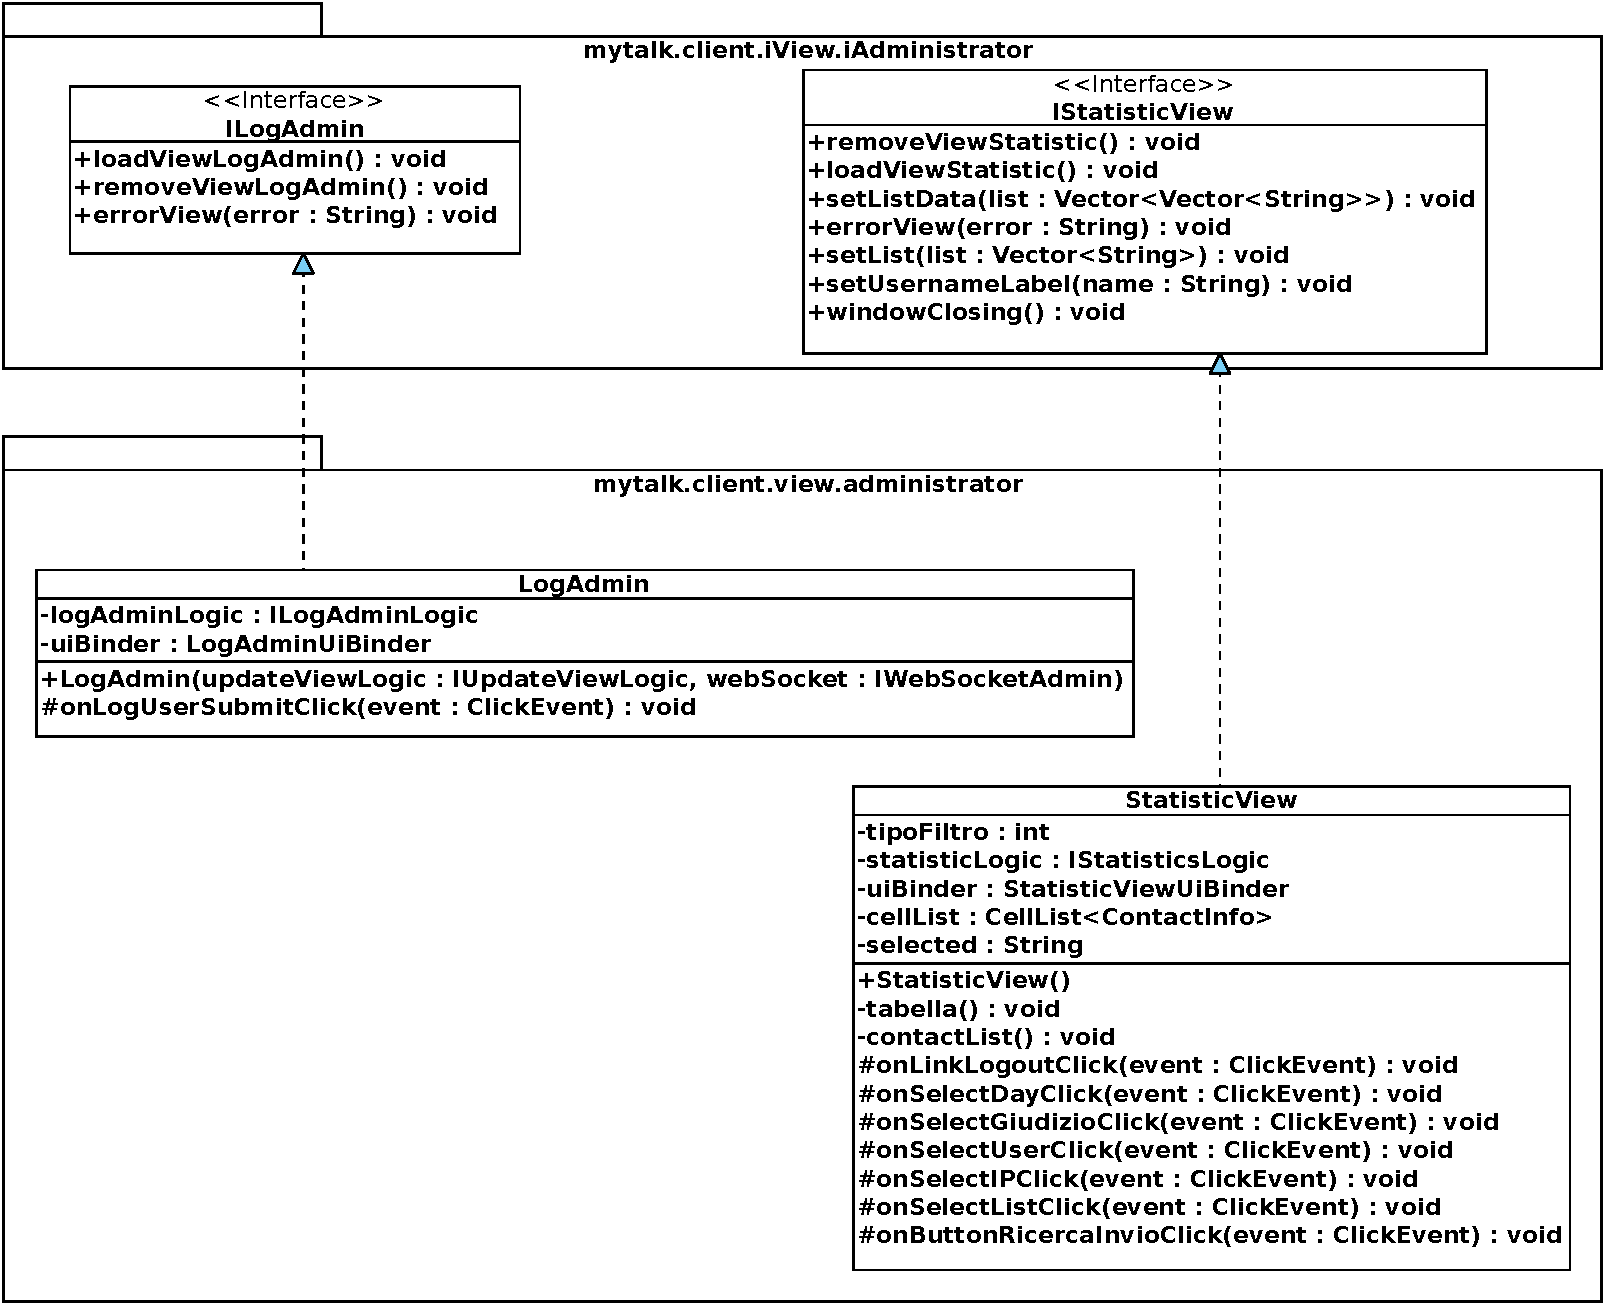
\includegraphics[scale=0.5]{\docsImg classi/statisticsView-logAdmin.pdf}
		\caption{Diagramma delle classi dei package \nolinkurl{mytalk.client.iView.iAdministrator} e  \nolinkurl{mytalk.client.view.administrator}; dettaglio delle classi \nolinkurl{ILogAdmin},  \nolinkurl{IStatisticView}, \nolinkurl{LogAdmin} e \nolinkurl{StatisticView}.}
	\end{figure}

		\begin{figure}[h!tbp]
		\centering
		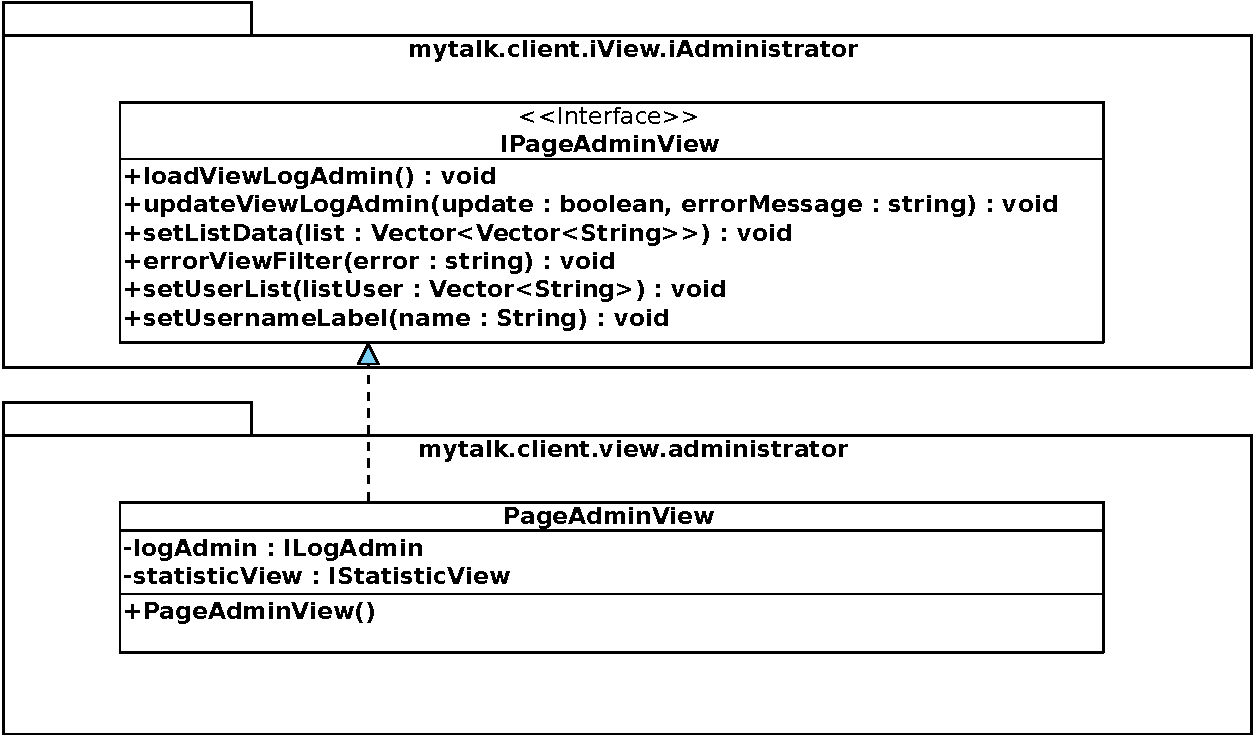
\includegraphics[scale=0.55]{\docsImg classi/pageAdminView.pdf}
		\caption{Diagramma delle classi dei package \nolinkurl{mytalk.client.iView.iAdministrator} e  \nolinkurl{mytalk.client.view.administrator}; dettaglio delle classi \nolinkurl{IPageAdminView} e \nolinkurl{PageAdminView}.}
	\end{figure}	
	
	
			% ILogAdmin - inizio
		\subsubsection{ILogAdmin}\label{ssub:ILogAdmin}{
			\begin{itemize}
				\item[]  \textbf{Funzione:} \\
				Interfaccia che offre operazioni alle classi che compongono la GUI\g~ per l'autenticazione degli amministratori e interagiscono con essa.\\
				
				\item[]  \textbf{Relazioni con altre componenti:} \\
				L'interfaccia è implementata da:
				\begin{itemize}
					\item[] \path{mytalk.client.view.administrator.LogAdmin}.
				\end{itemize}
				L'interfaccia è utilizzata da:
				\begin{itemize}
					\item[] \path{mytalk.client.view.adminstrator.PageAdminView}.\\
				\end{itemize}
				
				\item[]  \textbf{Metodi:}\\
				\texttt{+ void loadViewLogAdmin();}\\
				Visualizza la GUI\g~ di autenticazione e seleziona le impostazioni di default\g, i campi vuoti e l'errore (non visibile).\\

				\texttt{+ void removeViewLogAdmin();}\\
				Nasconde la GUI\g~ di autenticazione.\\

				\texttt{+ void errorView(String error);}\\
				Imposta e rende visibile il messaggio di errore.\\
			\end{itemize}
			}
		% ILogAdmin - fine
  
		% IPageAdminView - inizio
		\subsubsection{IPageAdminView}\label{ssub:IPageAdminView}{
	
			\begin{itemize}
				\item[]  \textbf{Funzione:} \\
				Interfaccia che offre operazioni alle classi che compongono la GUI\g~ e interagiscono con essa.\\
				
				\item[]  \textbf{Relazioni con altre componenti:} \\
				L'interfaccia è implementata da:
				\begin{itemize}
					\item[] \path{mytalk.client.view.administrator.PageAdminView}.
				\end{itemize}
				L'interfaccia è utilizzata da:
				\begin{itemize}
					\item[] \path{mytalk.client.MyTalkAdmin};
					\item[] \path{mytalk.client.presenter.administrator.logicAdmin.UpdateUserView}.\\
				\end{itemize}
				
				\item[]  \textbf{Metodi:}\\
					\texttt{+ void loadViewLogAdmin();}\\
					Richiede la visualizzazione della GUI\g~ di autenticazione dell'amministratore.\\
					
					\texttt{+ void updateViewLogAdmin(boolean update, String errorMessage);}\\
					Aggiorna la GUI\g~ a seconda del valore di \texttt{update}:
					\begin{itemize}
						\item[-] se \texttt{false}: aggiorna la GUI\g~ di autenticazione visualizzando l'errore opportuno contenuto in \texttt{errorMessage};
						\item[-] se \texttt{true}: rende invisibile la GUI\g~ di autenticazione e visualizza la GUI\g~ di visualizzazione delle statistiche.\\
					\end{itemize}
					
					\texttt{+ void setListData(Vector<Vector<String>> list);}\\
					Invia i dati delle statistiche alla tabella di visualizzazione.\\
					
					\texttt{+ void errorViewFilter(String error);}\\
					Notifica la presenza di errori nella chiave usata come filtro.\\
					
					\texttt{+ void setUserList(Vector<String> listaUtenti);}\\
					Imposta la lista degli utenti.\\
					
					\texttt{+ void setUsernameLabel(String name);}\\
					Invia il nome utente alla GUI\g~ di visualizzazione delle statistiche.\\
			\end{itemize}
			}
		% IPageAdminView - fine
		
		% IStatisticView - inizio
		\subsubsection{IStatisticView}\label{ssub:IStatisticView}{
			\begin{itemize}
				\item[]  \textbf{Funzione:} \\
				Offre operazioni alle classi che compongono la GUI\g~ per la visualizzazione delle statistiche da parte dell'amministratore e interagiscono con essa.\\
				
				\item[]  \textbf{Relazioni con altre componenti:} \\
				L'interfaccia è implementata da:
				\begin{itemize}
					\item[] \path{mytalk.client.view.administrator.StatisticView}.
				\end{itemize}
				L'interfaccia è utilizzata da:
				\begin{itemize}
					\item[] \path{mytalk.client.view.administrator.PageAdminView}.\\
				\end{itemize}

				\item[]  \textbf{Metodi:}\\
				\texttt{+ void removeViewStatistic();}\\
				Nasconde la GUI\g~ di visualizzazione statistiche.\\

				\texttt{+ void loadViewStatistic();}\\
				Visualizza la GUI\g~ che mostra le statistiche.\\
				
				\texttt{+ void setListData(Vector<Vector<String>> list);}\\
				Inserisce nella tabella contenente le statistiche i dati contenuti nel parametro \texttt{list}.\\
				
				\texttt{+ void errorView(String error);}\\
				Imposta e rende visibile il messaggio di errore.\\
				
				\texttt{+ void setList(Vector<String> list);}\\
				Inserisce gli utenti registrati contenuti nel vettore \texttt{list}.\\
				
				\texttt{+ void setUsenameLabel(String name);}\\
				Imposta l'etichetta \texttt{LabelUser} con il nome dell'amministratore autenticato.\\
				
				\texttt{+ void windowClosing();}\\
				Gestisce l'evento di chiusura della finestra della GUI\g~ di  visualizzazione delle statistiche effettuando il logout.\\
			\end{itemize}
			}
		% IStatisticView - fine
	}
	
	\subsection{Package mytalk.client.view.administrator} {
		
		% LogAdmin - inizio
		\subsubsection{LogAdmin}\label{ssub:LogAdmin}{
			\begin{itemize}
				\item[]  \textbf{Funzione:} \\
				La classe ha il compito di:
				\begin{itemize}
					\item[-] aggiornare opportunamente la GUI\g~ di autenticazione dell'amministratore;
					\item[-] Data di approvazione del file gestire gli eventi che l'utente o il sistema possono innescare inoltrando le richieste all'interfaccia \texttt{ILogAdminLogic}.\\
				\end{itemize}
				
				\item[]  \textbf{Relazioni con altre componenti:} \\
				Implementa l'interfaccia:
				\begin{itemize}
					\item[] \path{mytalk.client.iView.iAdministrator.ILogAdmin}.
				\end{itemize}
				Usa le classi:
				\begin{itemize}
		\item[]\path{mytalk.client.presenter.administrator.logicAdmin.LogAdminLogic}. 
				\end{itemize}
				Tramite le interfacce:
				\begin{itemize}
					\item[] \path{mytalk.client.iPresenter.iAdministrator.iLogicAdmin.ILogAdminLogic}.\\
				\end{itemize}

				\item[] \textbf{Attributi:}\\
					\texttt{- ILogAdminLogic logAdminLogic}: riferimento alla classe \texttt{LogAdminLogic}.\\
				
				\item[] \textbf{Oggetti:}\\
					\texttt{@UiField HTMLPanel MyDivLogin}: pannello contente \texttt{FormLogUser}.\\

					\texttt{@UiField FormPanel FormLogUser}: form contenente \texttt{BoxUtente}, \texttt{BoxPassword}, \texttt{LabelError} e \texttt{LogUserSubmit}.\\

					\texttt{@UiField TextBox BoxUtente}: campo per l'inserimento del nome utente.\\

					\texttt{@UiField TextBox BoxPassword}: campo per l'inserimento della password.\\

					\texttt{@UiField InlineLabel LabelError}: label che in presenza di errore ne segnala il tipo.\\

					\texttt{@UiField PushButton LogUserSubmit}: bottone per l'invio della richiesta di controllo delle credenziali di autenticazione dell'amministratore.\\
				
				\item[] \textbf{Metodi:}\\
					\texttt{+ LogAdmin(IUpdateViewLogic updateViewLogic, IWebSocketAdmin webSocket);}\\
					Costruttore: inizializza \texttt{logAdminLogic} con i valori ricevuti come parametri, imposta gli attributi degli oggetti che compongono la GUI\g~ e imposta come invisibile \texttt{LabelError}.\\

					\texttt{+ void loadViewLogAdmin();}\\
					Visualizza la GUI\g~ di autenticazione dell'amministratore e seleziona le impostazioni di default\g~: 
					\texttt{BoxUtente} e \texttt{BoxPassword} vuoti e \texttt{LabelError} invisibile.\\
					
					\texttt{+ void removeViewLogAdmin();}\\
					Nasconde la GUI\g~ di login.\\
					
					\texttt{+ void errorView(String error);}\\
					Imposta e rende visibile \texttt{LabelError} inserendo il contenuto della stringa \texttt{error}.\\
				
				\item[] \textbf{Eventi:}\\
					\texttt{@UiHandler void onLogUserSubmitClick(ClickEvent event);}\\
					All'evento \texttt{Click} dell'oggetto \texttt{LogUserSubmit} i dati inseriti all'interno dei campi \texttt{BoxUtente} e \texttt{BoxPassword} vengono inseriti in un vettore e inviati attraverso il riferimento \texttt{logAdminLogic} al metodo \texttt{validateData(Vector<String>)} per effettuare il controllo dei dati di autenticazione.\\
			\end{itemize}
			}
		% LogAdmin - fine

		% PageAdminView - inizio
		\subsubsection{PageAdminView}\label{ssub:PageAdminView}{
			\begin{itemize}
				\item[]  \textbf{Funzione:} \\
				La classe ha il compito di smistare le richieste di aggiornamento della View da parte del Presenter.\\
				
				\item[]  \textbf{Relazioni con altre componenti:} \\
				Implementa l'interfaccia:
				\begin{itemize}
					\item[] \path{mytalk.client.iView.iAdministrator.IPageAdminView}.
				\end{itemize}
				Usa le classi:
				\begin{itemize}
					\item[] \path{mytalk.client.view.administrator.LogAdminView};
					\item[] \path{mytalk.client.view.administrator.StatisticView};
					\item[] \path{mytalk.client.presenter.administrator.logicAdmin.UpdateViewLogic}.
				\end{itemize}
				Tramite le interfacce:
				\begin{itemize}
					\item[] \path{mytalk.client.iView.iAdministrator.ILogAdminView};
					\item[] \path{mytalk.client.iView.iAdministrator.IStatisticView};
					\item[] \path{mytalk.client.iPresenter.iAdministrator.iLogicAdmin.IUpdateViewLogic}.\\
				\end{itemize}
					
				\item[] \textbf{Attributi:}\\
					\texttt{- ILogAdmin logAdmin}: riferimento alla classe \texttt{LogAdmin};\\
					
					\texttt{- IStatisticView statisticView}: riferimento alla classe \texttt{StatisticView}.\\

				\item[] \textbf{Metodi:}\\
					\texttt{+ PageAdminView();}\\
					Costruttore:
					\begin{itemize}
						\item[-] inizializza, carica nel pannello di root e imposta la visibilità degli oggetti \texttt{logAdmin} e \texttt{statisticView};
						\item[-] imposta un listener che attende l'evento di chiusura della pagina e che in tal caso richiama i metodi di chiusura degli oggetti \texttt{statisticView}.\\
					\end{itemize}
					
					\texttt{+ void loadViewLogAdmin();}\\
					Richiama il metodo \texttt{loadViewLogAdmin()} attraverso il riferimento \texttt{logAdmin} per visualizzare l'autenticazione dell'amministratore.\\
					
					\texttt{+ void updateViewLogAdmin(boolean update, String errorMessage);}\\
					Aggiorna la GUI\g~ a seconda del valore \texttt{update}:
					\begin{itemize}
						\item[-] se \texttt{false}: richiama il metodo \texttt{errorView(message)} attraverso il riferimento \texttt{logAdmin} per visualizzare gli errori di autenticazione;
						\item[-] se \texttt{true}: richiama il metodo \texttt{removeViewLogAdmin()} attraverso il riferimento \texttt{logAdmin} e successivamente richiama il metodo \texttt{loadViewStatistic()} attraverso il riferimento \texttt{statisticView}.\\
					\end{itemize}
					
					\texttt{+ void setListData(Vector<Vector<String>> list);}\\
					Invia i dati delle statistiche alla tabella di visualizzazione con il metodo \texttt{setListData(list)} attraverso il riferimento \texttt{statisticView}.\\
					
					\texttt{+ void errorViewFilter(String error);}\\
					Richiama il metodo \texttt{errorView(messages)} attraverso il riferimento \texttt{statisticView} per visualizzare gli errori di filtro di ricerca.\\
					
					\texttt{+ void setUserList(Vector<String> listUser);}\\
					Richiama il metodo \texttt{setList(listaUtenti)} attraverso il riferimento \texttt{statisticView} per impostare la lista utenti del filtro di ricerca per lista.\\
					
					\texttt{+ void setUsernameLabel(String name);}\\
					Richiama il metodo \texttt{setUsenameLabel(name)} attraverso il riferimento \texttt{statisticView}.\\
			\end{itemize}
			}
		% PageAdminView - fine
		
		% StatisticView - inizio
		\subsubsection{StatisticView}\label{ssub:StatisticView}{
			\begin{itemize}
				\item[]  \textbf{Funzione:} \\
				La classe ha il compito di:
				\begin{itemize}
					\item[-] aggiornare opportunamente la GUI\g~ di visualizzazione delle statistiche;
					\item[-] gestire gli eventi che l'utente o il sistema possono innescare inoltrando le richieste all'interfaccia \texttt{IStatisticLogic};\\
				\end{itemize}
				
				\item[]  \textbf{Relazioni con altre componenti:} \\
				Implementa l'interfaccia:
				\begin{itemize}
					\item[] \path{mytalk.client.iView.iAdministrator.IStatisticView}.
				\end{itemize}
				Usa le classi:
				\begin{itemize}
					\item[] \path{mytalk.client.presenter.administrator.logicAdmin.StatisticLogic}.
				\end{itemize}
				Tramite le interfacce:
				\begin{itemize}
					\item[] \path{mytalk.client.iPresenter.iAdministrator.iLogicAdmin.IStatisticLogic}.\\
				\end{itemize}
					
				\item[] \textbf{Attributi:}\\
					\texttt{- IStatisticLogic statisticLogic}: riferimento alla classe \texttt{StatisticLogic};\\

					\texttt{- int tipoFiltro}: identifica il tipo di indice usato:
					\begin{itemize}
						\item[-] 1: giorno;
						\item[-] 2: giudizio;
						\item[-] 3: nome utente;
						\item[-] 4: IP\g~ (non attivo al momento);
						\item[-] 5: da lista. \\
					\end{itemize}

					\texttt{- CellList<ContactInfo> cellList}: identifica l'oggetto che contiene la lista degli utenti registrati.\\
					
					\texttt{- String selected}: string che identifica l'utente attualmente selezionato.\\
				
				\item[] \textbf{Oggetti:}\\
					\texttt{@UiField HTMLPanel MyDiv}: pannello contente \texttt{DivStatisticVision} e \texttt{DivPanelControl}.\\

					\texttt{@UiField HTMLPanel DivStatisticVision}: pannello contente \texttt{cellTable}.\\

					\texttt{@UiField CellTable<Vector<Vector<String>>}: tabella per la visualizzazione dei dati delle statistiche.\\

					\texttt{@UiField HTMLPanel DivPanelControl}: pannello contenente \texttt{LinkLogout}, \texttt{LabelUser} e \texttt{FormFiltro}.\\

					\texttt{@UiField InlineHyperlink LinkLogout}: link per passare alla GUI\g~ dell'autenticazione dell'amministratore effettuando il logout.\\

					\texttt{@UiField InlineLabel LabelUser:}: label che visualizza lo username dell'utente autenticato.\\

					\texttt{@UiField FormPanel FormFiltro}: form contente \texttt{GridFiltro}.\\

					\texttt{@UiField Grid GridFiltro}: griglia contenente \texttt{SelectDay}, \texttt{SelectGiudizio}, \texttt{SelectUser}, \texttt{SelectIP}, \texttt{SelectList}, \texttt{Aggiorna}, \texttt{ButtonRicercaInvio}, \texttt{LabelErrorRicerca}, \texttt{ListBoxUtenti}.\\

					\texttt{@UiField PushButton SelectDay}: bottone per impostare il valore di \texttt{tipoFiltro} a 1 e rendere visibili \texttt{BoxRicerca} e \texttt{ButtonRicercaInvio}.\\

					\texttt{@UiField PushButton SelectGiudizio}: bottone per impostare il valore di \texttt{tipoFiltro} a 2 e rendere visibili \texttt{BoxRicerca} e \texttt{ButtonRicercaInvio}.\\

					\texttt{@UiField PushButton SelectUser}: bottone per impostare il valore di \texttt{tipoFiltro} a 3 e rendere visibili \texttt{BoxRicerca} e \texttt{ButtonRicercaInvio}.\\

					\texttt{@UiField PushButton SelectIP}: bottone per impostare il valore di \texttt{tipoFiltro} a 4 e rendere visibili \texttt{BoxRicerca} e \texttt{ButtonRicercaInvio}.\\

					\texttt{@UiField PushButton SelectList}: bottone per impostare il valore di \texttt{tipoFiltro} a 5 e rendere visibili \texttt{ListBoxUtenti} e \texttt{ButtonRicercaInvio}.\\

					\texttt{@UiField PushButton Aggiorna}: bottone per inviare la richiesta di aggiornamento di \texttt{cellTable} e impostare invisibili \texttt{ListBoxUtenti}, \texttt{BoxRicerca} e \texttt{ButtonRicercaInvio}.\\

					\texttt{@UiField PushButton ButtonRicercaInvio}: bottone per richiedere di filtrare i dati di \texttt{cellTable} a seconda del tipo di filtro e della chiave inserita in \texttt{BoxRicerca} o \texttt{ListBoxUtenti}.\\

					\texttt{@UiField InlineLabel LabelErrorRicerca}: label che contiene l'errore relativo alla ricerca della chiave usata da \texttt{filtro}.\\

					\texttt{@UiField ListBox ListBoxUtenti}: oggetto contenente la lista di tutti gli utenti registrati.\\

					\texttt{@UiField TextBox BoxRicerca}: campo per l'inserimento della chiave da usare come filtro.\\
				
				\item[] \textbf{Metodi:}\\
					\texttt{+ StatisticView(IUpdateViewLogic updateViewLogic, IWebSocketAdmin webSocket);}\\
					Costruttore: inizializza \texttt{communicationLogic} con i valori ricevuti come parametri, imposta inoltre \texttt{webSocket} con il valore del riferimento \texttt{statisticLogic}. Imposta gli attributi degli oggetti che compongono la GUI\g~ e crea le colonne di \texttt{cellTable} attraverso il metodo \texttt{tabella()}.\\

					\texttt{+ void removeViewStatistic();}\\
					Nasconde la GUI\g~ di visualizzazione statistiche.\\
					
					\texttt{+ void loadViewStatistic();}
					\begin{itemize}
						\item[-] visualizza la GUI\g~ di comunicazione e imposta come attivi tutti i filtri;
						\item[-] richiama il metodo \texttt{setUsernameLabel()} attraverso il riferimento \texttt{statisticLogic};
						\item[-] imposta visibile la tabella;
						\item[-] richiama il metodo \texttt{getListData()} attraverso il riferimento \texttt{statisticLogic} per richiedere di popolare la tabella.\\
					\end{itemize}
					
					\texttt{+ void setListData(Vector<Vector<String>> list);}\\
					Popola la tabella con le statistiche i dati contenuti nel parametro \texttt{list}.\\
					
					\texttt{+ void errorView(String error);}\\
					Rende visibile il messaggio di errore.\\
					
					\texttt{+ void setList(Vector<String> list);}\\
					Inserisce gli utenti registrati contenuti nel vettore \texttt{list} e li inserisce all'interno degli oggetti contenuti in \texttt{cellList}.\\
					
					\texttt{+ void setUsenameLabel(String name);}\\
					Imposta l'etichetta \texttt{LabelUser} con il nome dell'amministratore autenticato.\\
					
					\texttt{+ void windowClosing();}\\
					Gestisce l'evento di chiusura della finestra della GUI\g~ di visualizzazione delle statistiche effettuando il logout.\\
					
					\texttt{- void tabella();}\\
					Metodo per la creazione delle colonne di \texttt{cellTable}.\\
					
					\texttt{- void contactList();}\\
					Metodo che crea l'oggetto \texttt{cellList} che contiene la lista delle celle contenenti le informazioni dei contatti.
				
				\item[] \textbf{Eventi:}\\
					\texttt{@UiHandler void onLinkLogoutClick(ClickEvent event);}\\
					All'evento \texttt{Click} dell'oggetto \texttt{LinkLogout} viene richiamato il metodo \texttt{removeViewStatistic()}. Inoltre utilizza il riferimento \texttt{communicationLogic} per effettuare il logout e richiamare la GUI\g~ di autenticazione attraverso il metodo \texttt{logoutUser()}.\\
					
					\texttt{@UiHandler void onSelectDayClick(ClickEvent event);}\\
					All'evento \texttt{Click} dell'oggetto \texttt{SelectDay} viene impostato \texttt{tipoFiltro} a 1. Viene disabilitato il bottone \texttt{SelectDay} e vengono resi visibili \texttt{BoxRicerca} e \texttt{ButtonRicercaInvio}.\\
					
					\texttt{@UiHandler void onSelectGiudizioClick(ClickEvent event);}\\
					All'evento \texttt{Click} dell'oggetto \texttt{SelectGiudizio} viene impostato \texttt{tipoFiltro} a 2. Viene disabilitato il bottone \texttt{SelectGiudizio} e vengono resi visibili \texttt{BoxRicerca} e \texttt{ButtonRicercaInvio}.\\
					
					\texttt{@UiHandler void onSelectUserClick(ClickEvent event);}\\
					All'evento \texttt{Click} dell'oggetto \texttt{SelectUser} viene impostato \texttt{tipoFiltro} a 3. Viene disabilitato il bottone \texttt{SelectUser} e vengono resi visibili \texttt{BoxRicerca} e \texttt{ButtonRicercaInvio}.\\
					
					\texttt{@UiHandler void onSelectIPClick(ClickEvent event);}\\
					All'evento \texttt{Click} dell'oggetto \texttt{SelectIP} viene impostato \texttt{tipoFiltro} a 4. Viene disabilitato il bottone \texttt{SelectIP} e vengono resi visibili \texttt{BoxRicerca} e \texttt{ButtonRicercaInvio}.\\
					
					\texttt{@UiHandler void onSelectListClick(ClickEvent event);}\\
					All'evento \texttt{Click} dell'oggetto \texttt{SelectList} viene impostato \texttt{tipoFiltro} a 5. Viene disabilitato il bottone \texttt{SelectList} e vengono resi visibili \texttt{BoxRicerca} e \texttt{ButtonRicercaInvio}.\\
					
					\texttt{@UiHandler void onAggiornaClick(ClickEvent event);}\\
					All'evento \texttt{Click} dell'oggetto \texttt{Aggiorna} vengono abilitati tutti i bottoni \texttt{Select} e vengono nascosti \texttt{ListBoxUtenti}, \texttt{BoxRicerca} e \texttt{ButtonRicercaInvio}. Inoltre viene richiamato il metodo \texttt{getListData()} attraverso il riferimento \texttt{statisticLogic}.\\
					
					\texttt{@UiHandler void onButtonRicercaInvioClick(ClickEvent event)}\\
					All'evento \texttt{Click} dell'oggetto \texttt{ButtonRicercaInvio} viene controllato il tipo di filtro e invocato il metodo \texttt{ricerca(chiave, tipoFiltro)} attraverso il riferimento \texttt{statisticLogic}.\\
			\end{itemize}
			}
		% StatisticView - fine
	}
}
\end{sloppypar}
}

